\documentclass[a4paper, 11pt, titlepage, twoside, openany]{book}
\usepackage{plain}
\usepackage{setspace}
% Layout
\usepackage[
  paperheight=29.7cm,
  paperwidth=21cm,
  outer=1.5cm,
  inner=2.5cm,
  top=2cm,
  bottom=2cm
]{geometry}
% Chapter
\usepackage{titlesec}
\singlespacing
\setcounter{secnumdepth}{3}
\setcounter{tocdepth}{3}
% Letter
\usepackage[utf8]{inputenc}
% Language
\usepackage[english]{babel}
% PDF/A
\usepackage[a-1b]{pdfx}
% Image
\usepackage{graphicx}
\usepackage{wrapfig}
\usepackage{stackengine}
\usepackage{etoolbox}
% For professional tables
\usepackage{tabularx}
\usepackage{booktabs}
\BeforeBeginEnvironment{wrapfigure}{\setlength{\intextsep}{0pt}}
\usepackage{subcaption} % Required for subfigures and subcaptions
% Hyperlink
\usepackage{xurl}
\usepackage[pdfa]{hyperref}
\hypersetup{breaklinks=true}
% Quotes
\usepackage{fvextra}   % must come before csquotes
\usepackage{csquotes}
\MakeOuterQuote{"}
% List
\usepackage{enumitem}
% Math
\usepackage{amsmath}
% Cref
\usepackage[capitalize]{cleveref}
% Use the algorithm2e package with options for line numbering, rules, and vertical lines
\usepackage[linesnumbered,ruled,vlined,nofillcomment]{algorithm2e}
% Colors
\usepackage[svgnames]{xcolor}
% Code listings
\usepackage{minted}
\usemintedstyle{friendly}
\definecolor{codebg}{rgb}{0.97,0.97,0.97}
\setminted{
  fontsize=\small,
  %baselinestretch=1.1,
  %linenos,
  breaklines,
  frame=lines,
  framesep=2mm,
  bgcolor=codebg,
}

\crefname{algocfline}{line}{lines}
\Crefname{algocfline}{Line}{Lines}
\crefname{algocf}{algorithm}{algorithms}
\Crefname{algocf}{Algorithm}{Algorithms}
\crefrangelabelformat{Section}{#3#1#4--#5\crefstripprefix{#1}{#2}#6}

\newcommand{\rowptr}{\texttt{row\_ptr}}
\newcommand{\colidx}{\texttt{col\_idx}}
\newcommand{\bigO}[1]{\ensuremath{\mathcal{O}(#1)}}
\newcommand{\amd}{\texttt{Amd}}
\newcommand{\pioneer}{\texttt{Pioneer}}
\newcommand{\grace}{\texttt{Grace}}
\newcommand{\chunksize}{\texttt{CHUNK\_SIZE}}
\newcommand{\gapbs}{\texttt{gapbs}}
\newcommand{\openmp}{\texttt{openmp}}
\newcommand{\pthreads}{\texttt{pthreads}}

% Document
\begin{document}
  % Cover
  \pagenumbering{gobble}
  \pagestyle{plain}
\thispagestyle{empty}

\begin{center}
  \begin{figure}[h!]
    \centering
    
\includegraphics[width=.6\textwidth]{images/logo/unitn.png}
  \end{figure}

  \vspace{2 cm}
  \LARGE{Department of Information Engineering and Computer Science\\}

  \vspace{1 cm}
  \Large{Bachelor's Degree in\\ Computer, Communication and Electronic Engineering}

  \vspace{2 cm}
  \Large\textsc{Final Dissertation\\}
  \vspace{1 cm}
  \Huge\textsc{Optimizing Breadth-First Search on Modern Energy-Efficient Multicore CPUs\\}
  \vspace{0.5 em}
  \Large{\textit{}} % Subtitle

  \vspace{2 cm}
  \begin{tabular*}{\textwidth}{c @{\extracolsep{\fill}} c}
    \Large{Supervisor}    & \Large{Student}      \\
    \Large{Flavio Vella}  & \Large{Salvatore D.  Andaloro} \\
    \Large{Co-Supervisor} & \Large{Mat. 000000}       \\
    \Large{Thomas Pasquali}  & {}                   \\
  \end{tabular*}

  \vspace{2 cm}
  \Large{Academic year 2024/2025}
\end{center}
  \clearpage

  % Acknowledgements
  \thispagestyle{empty}

\begin{center}
  {\bf \LARGE Acknowledgments}
\end{center}

\vspace{2mm}
\emph{
I would like to thank my co-supervisor and friend Thomas, for his invaluable help in supporting the development of this project and for providing the original motivation for this thesis. My sincere thanks to Prof. Vella for his insightful advice and guidance, and to all the other university professors and staff who have contributed to my education.
}
\par
\emph{
To my wonderful family, I offer my heartfelt appreciation for their unwavering support, for providing me with a great education and immense warmth, and to all my friends for their help, counsel, and the joyful times we have shared and will share.
}

\vspace{1cm}

\begin{center}
    {\bf \LARGE Ringraziamenti}
\end{center}

\vspace{2mm}

\emph{
Vorrei ringraziare il mio correlatore e amico Thomas, per il suo prezioso aiuto nel seguire lo sviluppo di questo progetto e per avermi dato lo spunto iniziale di questa tesi. Desidero inoltre ringraziare il Prof. Vella per i suoi consigli e la sua guida, e tutti gli altri professori e il personale universitario che hanno contribuito alla mia formazione.
}
\par
\emph{
Desidero ringraziare di cuore la mia splendida famiglia, per l’affetto e la fiducia con cui mi ha sempre sostenuto e per avermi sempre garantito un’istruzione di qualità. Inoltre, vorrei ringraziare i miei amici per il loro sostegno, i loro consigli e i momenti felici che abbiamo condiviso e che condivideremo.
}
  \clearpage
  \pagestyle{plain}

  % Table of Contents
  \frontmatter
  \pagenumbering{Roman}
  \tableofcontents
  \clearpage
  \begingroup
  \pagestyle{empty}
  \cleardoublepage
  \endgroup

  % Start page numbering
  \mainmatter

  % Group to define space between chapters
  \begingroup
  % Override format of title chapter
  \titleformat{\chapter} {\normalfont\Huge\bfseries}{\thechapter}{1em}{} \titlespacing*{\chapter}{0pt}{0.59in}{0.02in}
  \titlespacing*{\section}{0pt}{0.20in}{0.02in} \titlespacing*{\subsection}{0pt}{0.10in}{0.02in}
  \titlespacing*{\subsubsection}{0pt}{0.05in}{0.02in}

  % Abstract
  \chapter*{Abstract}
\label{cha:abtract}
\addcontentsline{toc}{chapter}{Abstract}
Breadth-First Search (BFS) is a fundamental algorithm for graph analysis, but its performance on modern multicore CPUs is generally limited by irregular memory access. The non-contiguous memory accesses inherent in traversing large-scale graphs lead to poor cache utilization and high-latency memory stalls, creating a significant performance bottleneck for parallel implementations. This thesis investigates and implements two distinct optimization strategies for parallel BFS, targeting modern energy-efficient multicore architectures and focusing on large-diameter graphs, such as road networks.

The first contribution is a cache-optimized implementation in C++ with OpenMP, which proposes a novel MergedCSR data structure. By co-locating vertex metadata with its adjacency list, this format enhances spatial locality to reduce cache misses. The second contribution is an explicitly parallelized implementation in C with pthreads, which provides fine-grained control over the execution model. This version employs a persistent thread pool, a chunk-based frontier with dynamic work-stealing for load balancing, and a lightweight, custom barrier for scalable synchronization.

Both implementations were evaluated against the GAP Benchmark Suite on a diverse set of graphs across x86, RISC-V, and ARM platforms. The results demonstrate that the MergedCSR data structure significantly improves memory performance, enabling a geomean speedup of up to 1.5x over the baseline on large-diameter graphs. Furthermore, the explicit pthreads implementation exhibits superior scalability due to its custom synchronization and outperforms the GAP benchmark with a geomean of 2.28x on road networks and 1.87x on random geometric graphs. This work concludes that achieving optimal performance for memory-bound graph algorithms requires a holistic approach: combining cache-aware data structure design with a fine-grained parallel execution model with low-overhead synchronization.

  % Chapters
  \section{Introduction}

\begin{frame}{Breadth-First Search}
    \begin{itemize}
        \item Breadth-First Search is a fundamental algorithm in graph analysis
        \item Used in many algorithms: Dijkstra, Maximum Flow, MSP...
        \item Vertices are labeled based on the \alert{distance} from a given \textit{source} vertex
    \end{itemize}
    \begin{figure}
        \centering
        \begin{subfigure}[b]{0.32\textwidth}
            \centering
            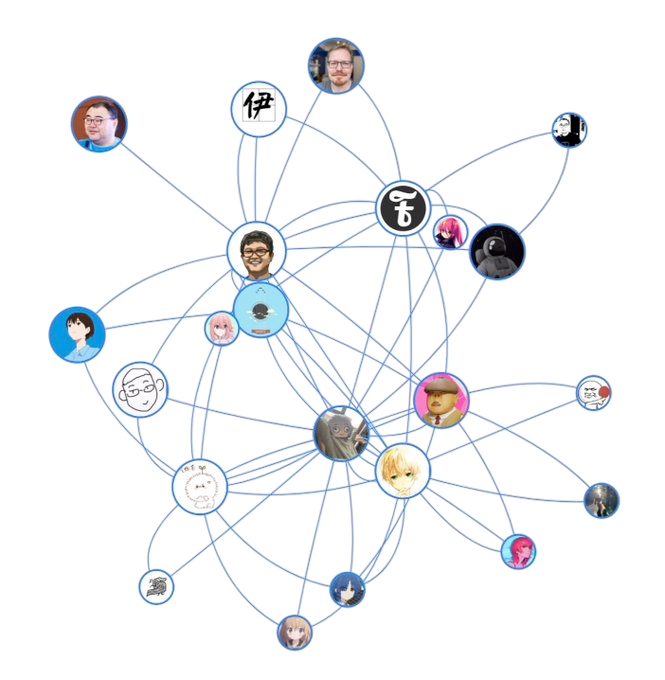
\includegraphics[width=0.8\linewidth]{images/Collaboration network.png}
            \caption{Social network}
        \end{subfigure}
        \begin{subfigure}[b]{0.32\textwidth}
            \centering
            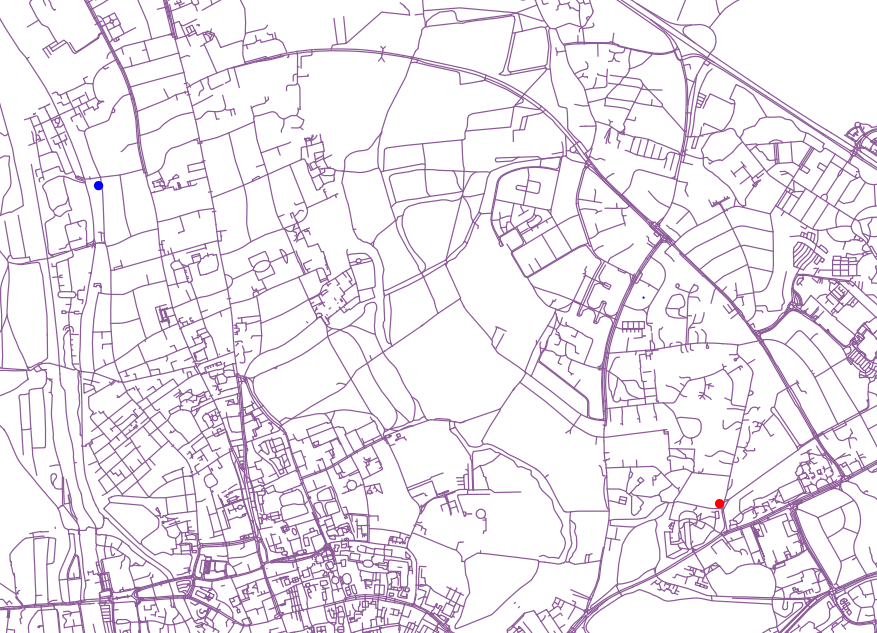
\includegraphics[width=1.05\linewidth]{images/roadnet.png}
            \caption{Road network}
        \end{subfigure}
    \end{figure}
\end{frame}

\begin{frame}{Breadth-First Search Example}
\centering
\begin{tikzpicture}[
    every node/.style={circle, draw},
    node distance=1.5cm,
  ]

  % Nodes
  \node[fill=white] (A) {A};
  \node[right=of A, fill=white] (B) {B};
  \node[below=of B, fill=white] (C) {C};
  \node[right=of B, fill=white] (D) {D};

  % Edges
  \draw (A) -- (B);
  \draw (A) -- (C);
  \draw (B) -- (C);
  \draw (B) -- (D);

  % Animations
  \uncover<2->{
    \node[fill=myred] (A) {A};
    \node[draw=myred, left=0.2cm of A, rectangle, align=center, font=\footnotesize] (boxA) {Distance = 0\\Parent = NULL};
  }

  \uncover<3->{
    \node[fill=myblue] (B) [right=of A] {B};
    \node[fill=myyellow] (C) [below=of B] {C};
    \node[draw=myblue, above=0.2cm of B, rectangle, align=center, font=\footnotesize] (boxB) {Distance = 1\\Parent = A};
    \node[draw=myyellow, below=0.2cm of C, rectangle, align=center, font=\footnotesize] (boxC) {Distance = 1\\Parent = A};
  }

  \uncover<4->{
    \node[fill=mygreen] (D) [right=of B] {D};
    \node[draw=mygreen, below=0.2cm of D, rectangle, align=center, font=\footnotesize] (boxD) {Distance = 2\\Parent = B};
  }
\end{tikzpicture}
\begin{minipage}{\textwidth}
    \centering
    \vspace{0.5cm}
    \only<1>{\textbf{Source vertex:} A}
    \only<2>{\textbf{Frontier:} A}
    \only<3>{\textbf{Frontier:} B, C}
    \only<4>{\textbf{Frontier:} D}
\end{minipage} 
\end{frame}

\begin{frame}{Modern Computer Architectures}
\begin{itemize}
    \item BFS has \bigO{V + E} time and space complexity (under RAM model)
    \item<2-> In practice, it is a \textbf{memory-bound algorithm} % no actual computation happening
    \begin{itemize}
        \item Algorithm exhibits poor cache locality
    \end{itemize}
    \item<3-> CPUs exhibit growing amount of \textbf{parallelism}...
    \item<4-> ...and new architectures are coming to the market (ARM, RISC-V)
\end{itemize}
\uncover<3->{
\begin{figure}
    \centering
    \vspace{-3mm}
    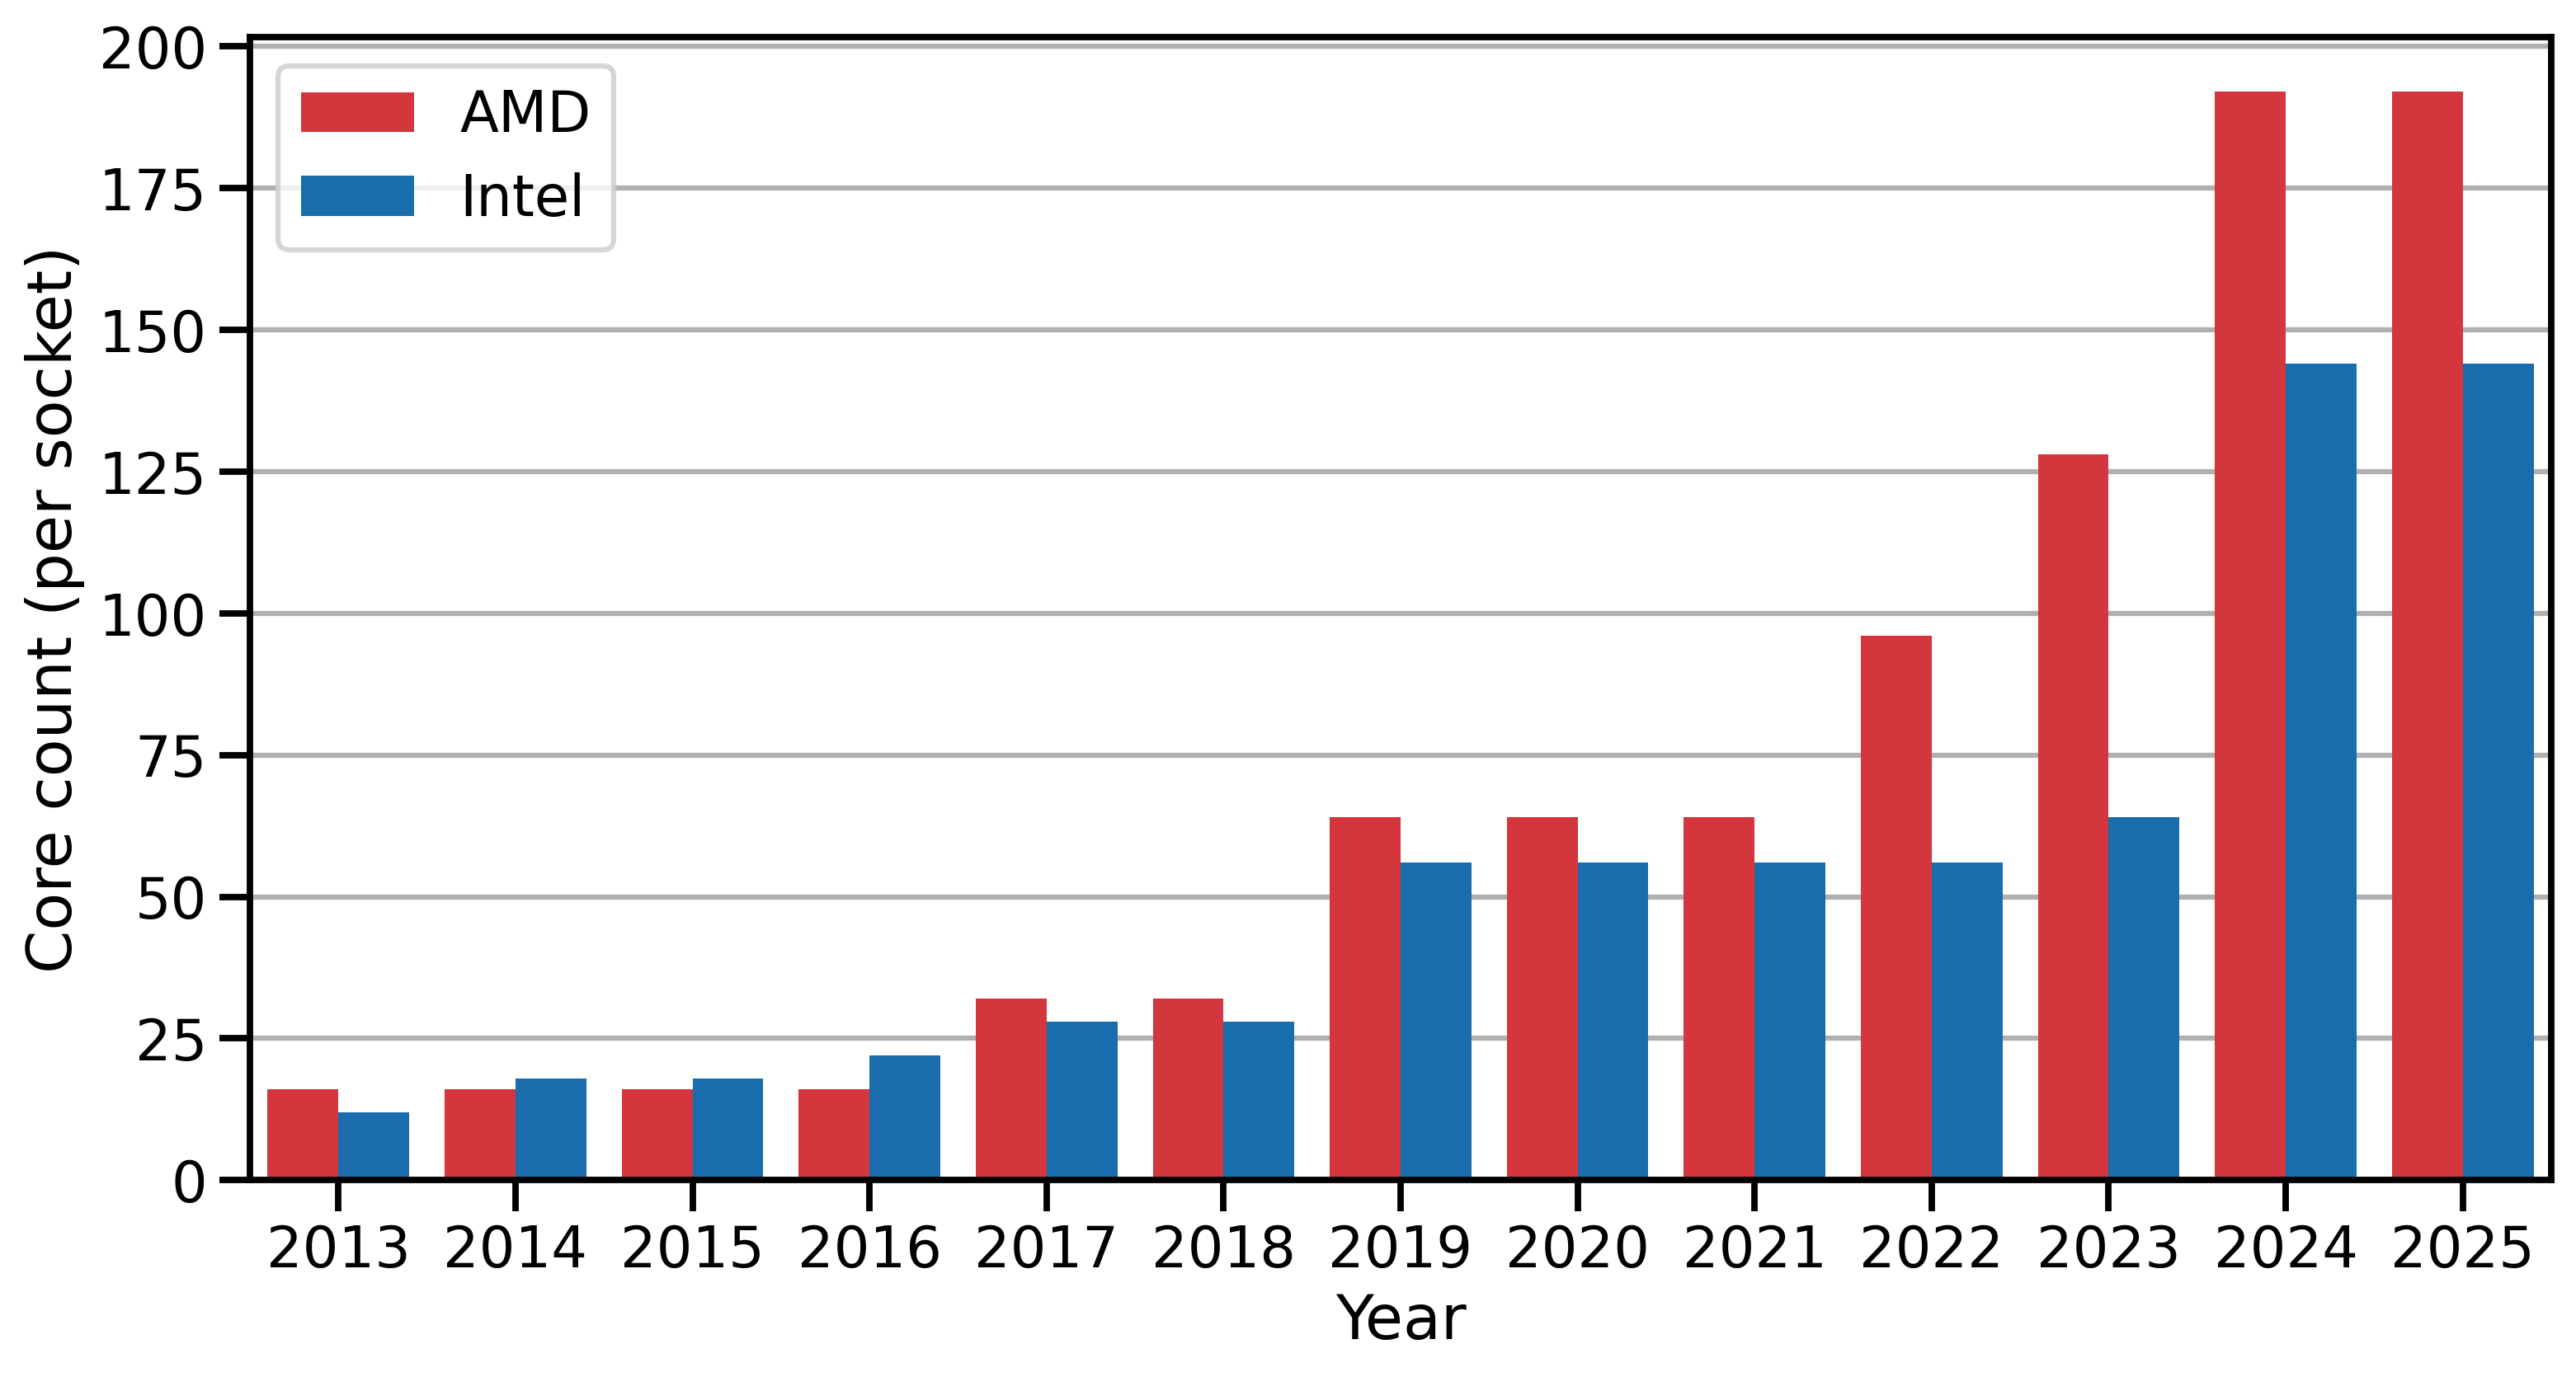
\includegraphics[width=0.6\linewidth]{images/cores.png}
    \vspace{-4mm}
    \caption{\scriptsize Evolution of core counts per socket for AMD and Intel processors}
    \label{fig:cores}
\end{figure}
}
\end{frame}

\begin{frame}{Contents}
\begin{itemize}
    \item New \textit{MergedCSR} data structure
    \item Two optimized parallel implementations (OpenMP and pthreads)
    \pause
    \item Evaluated against GAP Benchmark suite
    \item Speedups compared on three different architectures (AMD x86, RISC-V, ARM)
\end{itemize}
\begin{figure}
    \centering
    \begin{subfigure}[c]{0.4\textwidth}
    \centering
        
\includegraphics[height=2.5cm]{images/gapbs.png}
        \caption{GAP suite logo}
    \end{subfigure}
    \begin{subfigure}[c]{0.4\textwidth}
        \centering
        
\includegraphics[height=2.5cm]{images/architectures.png}
        \caption{Compared architectures}
    \end{subfigure}
\end{figure}
\end{frame}
  \chapter{Background}
Despite the algorithmic simplicity of BFS, achieving high performance execution is a significant challenge on modern multi-core architectures. The primary performance bottleneck is not the algorithm's asymptotical computational complexity, which is linear in the number of vertices and edges, but rather its memory access pattern. The irregular and unpredictable structure of most real-world graphs results in non-contiguous memory accesses, which leads to poor cache utilization and high-latency stalls as the processor waits for data to be fetched from main memory \cite{lenharth2016parallel, lumsdaine2007challenges}. Consequently, state-of-the-art research has largely focused on two areas: refining the traversal strategy itself \cite{arai2024doubling, beamer2013direction, jia2012edge} and redesigning the underlying graph data structures to be more amenable to the memory hierarchies of modern hardware \cite{torok2020improving, iwabuchi2014nvm}.

\section{Direction-Optimizing BFS}
A pivotal advancement in traversal strategy was the introduction of direction-optimizing or Hybrid BFS, proposed by Beamer et al. in 2012 \cite{beamer2013direction}. In a Breadth-First Search, the set of vertices at the current depth of the search is known as the frontier. In this strategy, each frontier expansion is approached either using the Top-Down approach or the Bottom-Up approach. The Top-Down approach, which was used in the other BFS algorithms prior to this work, involves each vertex in the current frontier exploring its neighbors to identify unvisited vertices, which then form the frontier for the next level. The Bottom-Up approach instead inverts the search. It iterates through all vertices and, for those that have not been visited, it checks if they have a parent in the current frontier. A visual representation of both strategies is shown in \cref{fig:hybrid_bfs}. 

\begin{figure}[h]
    \centering
    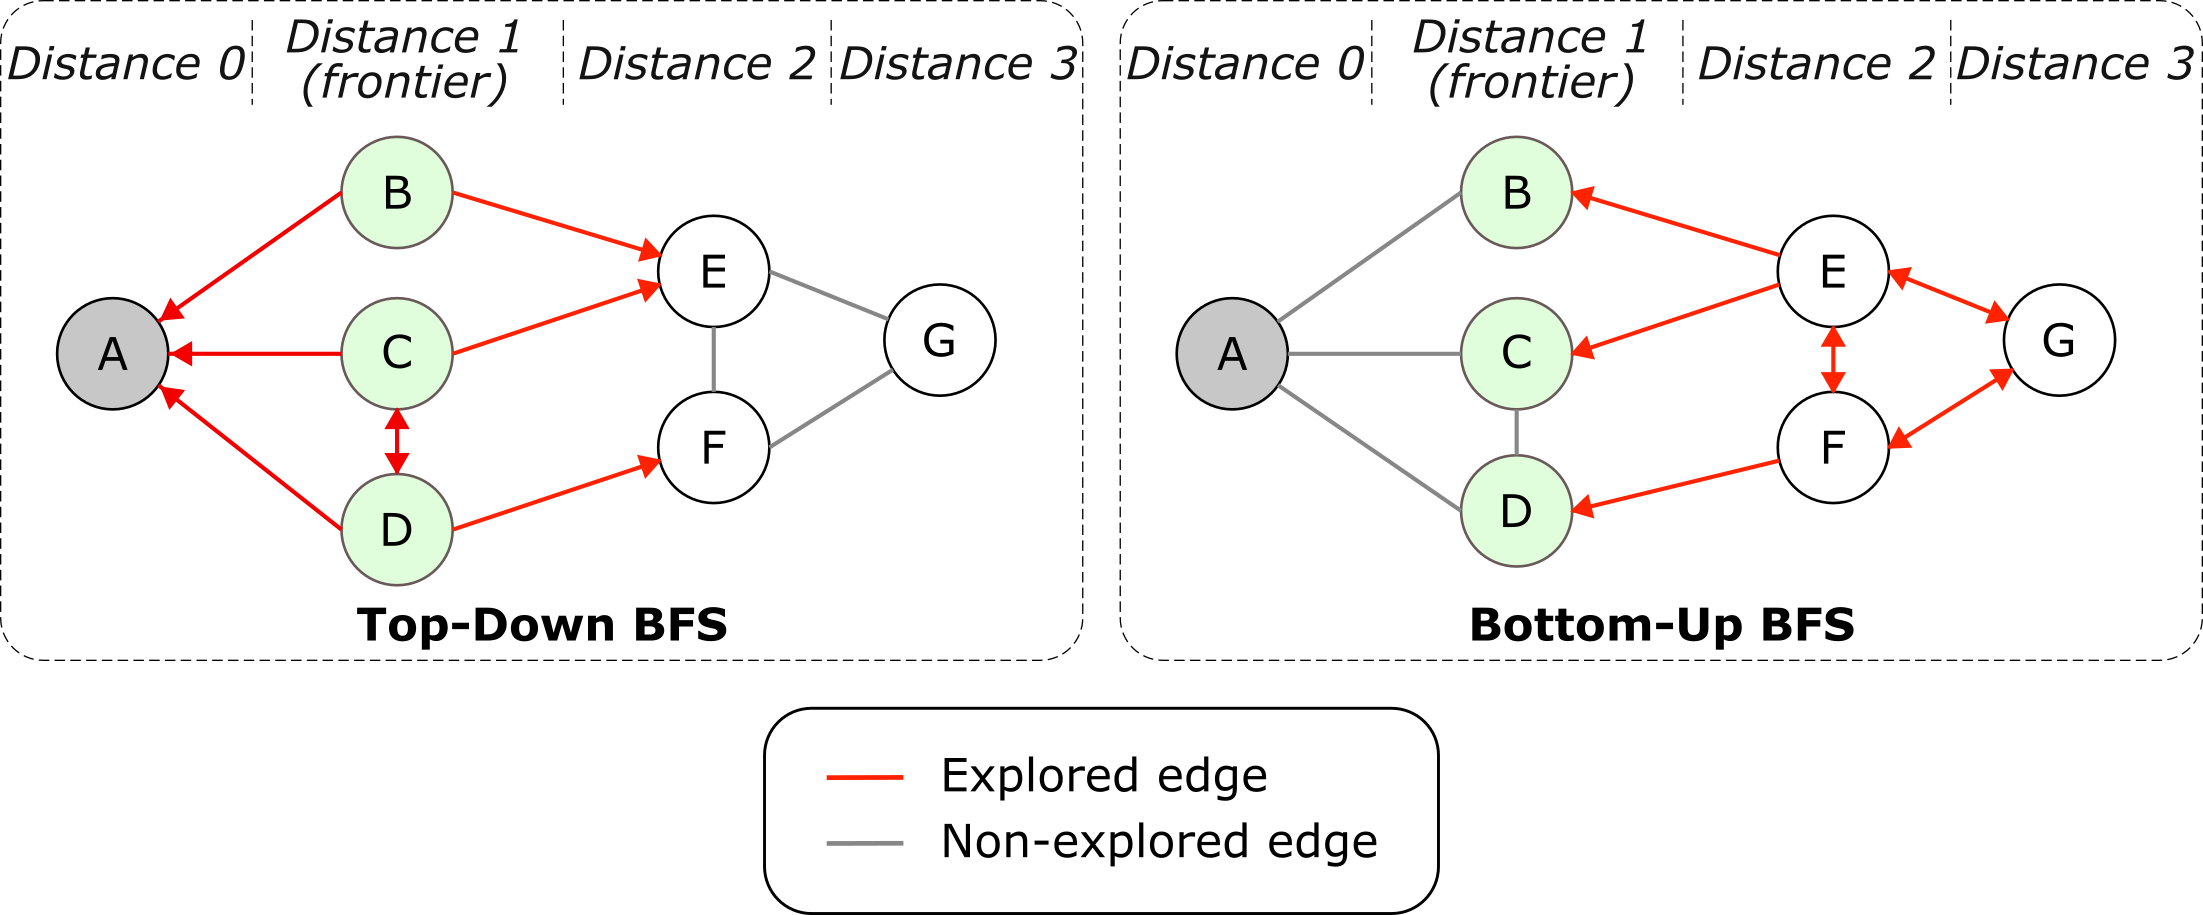
\includegraphics[width=0.8\linewidth]{images/hybrid bfs.png}
    \caption{Comparison of Top-Down and Bottom-Up Breadth-First Search strategies, starting from source vertex A, for discovering vertices at distance 2. The frontier is the set of vertices at distance 1 $\{B, C, D\}$. The Top-Down approach inspects the neighbors of each vertex in the frontier. This process requires 8 edge traversals to find the next level. However, this strategy performs some superfluous work: it revisits the already visited vertex A, it redundantly traverses the edge C-E even though E was already discovered through B-E, and it unnecessarily traverses edge C-D  and D-C. In contrast, the Bottom-Up approach inspects all unexplored vertices $\{E,F,G\}$, and checks whether any of their neighbors belong to the current frontier $\{B,C,D\}$. This method requires 9 edge traversals, since edges between unexplored vertices (such as E-F, E-G, and F-G) are traversed in both directions.}
    \label{fig:hybrid_bfs}
\end{figure}

\section{Graph diameter and frontier expansions}
The effectiveness of the Top-Down and Bottom-Up strategies is intrinsically linked to a graph's structural properties, most notably its diameter. The diameter dictates the shape and size of the BFS frontier at each level of the traversal, which is the primary factor in determining the most efficient approach \cite{beamer2013direction, andaloro2025cache, arai2024doubling}. This relationship gives rise to two broad classes of graphs: small-diameter and large-diameter.

Small-Diameter Graphs, such as the social networks shown in the plot, are characterized by the "small-world" phenomenon \cite{amaral2000classes}. The frontier size exhibits a distinct pattern: it quickly grows to encompass a significant fraction of the total vertices, and then rapidly collapses. For these graphs, a hybrid traversal is essential. The Top-Down strategy is efficient for the initial and final levels, but during the intermediate phase where the frontier is massive, the Bottom-Up strategy is superior, because it is more efficient to have the small set of unvisited nodes "find" the enormous frontier than the other way around.

Large-Diameter Graphs, such as road networks, Finite Element Models, and Random Geometric Graphs, lack vertices with high degree that create short paths. Consequently, the BFS frontier progresses in a slow, wave-like manner, never "exploding" in size. As shown in the figure, the frontier size for the road networks, FEM and RGG graphs remains relatively small throughout the entire, much longer traversal (the y-axis is logarithmic). For these graphs, the Top-Down approach is almost always the more efficient strategy, as the number of outgoing edges from the frontier is never large enough to justify the high overhead of a Bottom-Up search, which would require iterating over the vast set of unvisited vertices at each step.

This dichotomy in frontier behavior is the core motivation for the direction-optimizing algorithm. The heuristics used to switch between the two modes try to dynamically classify the state of the traversal at each level, applying the Bottom-Up optimization only when the frontier grows large enough to resemble the intermediate state of a small-diameter graph traversal.

\begin{figure}[h]
    \centering
    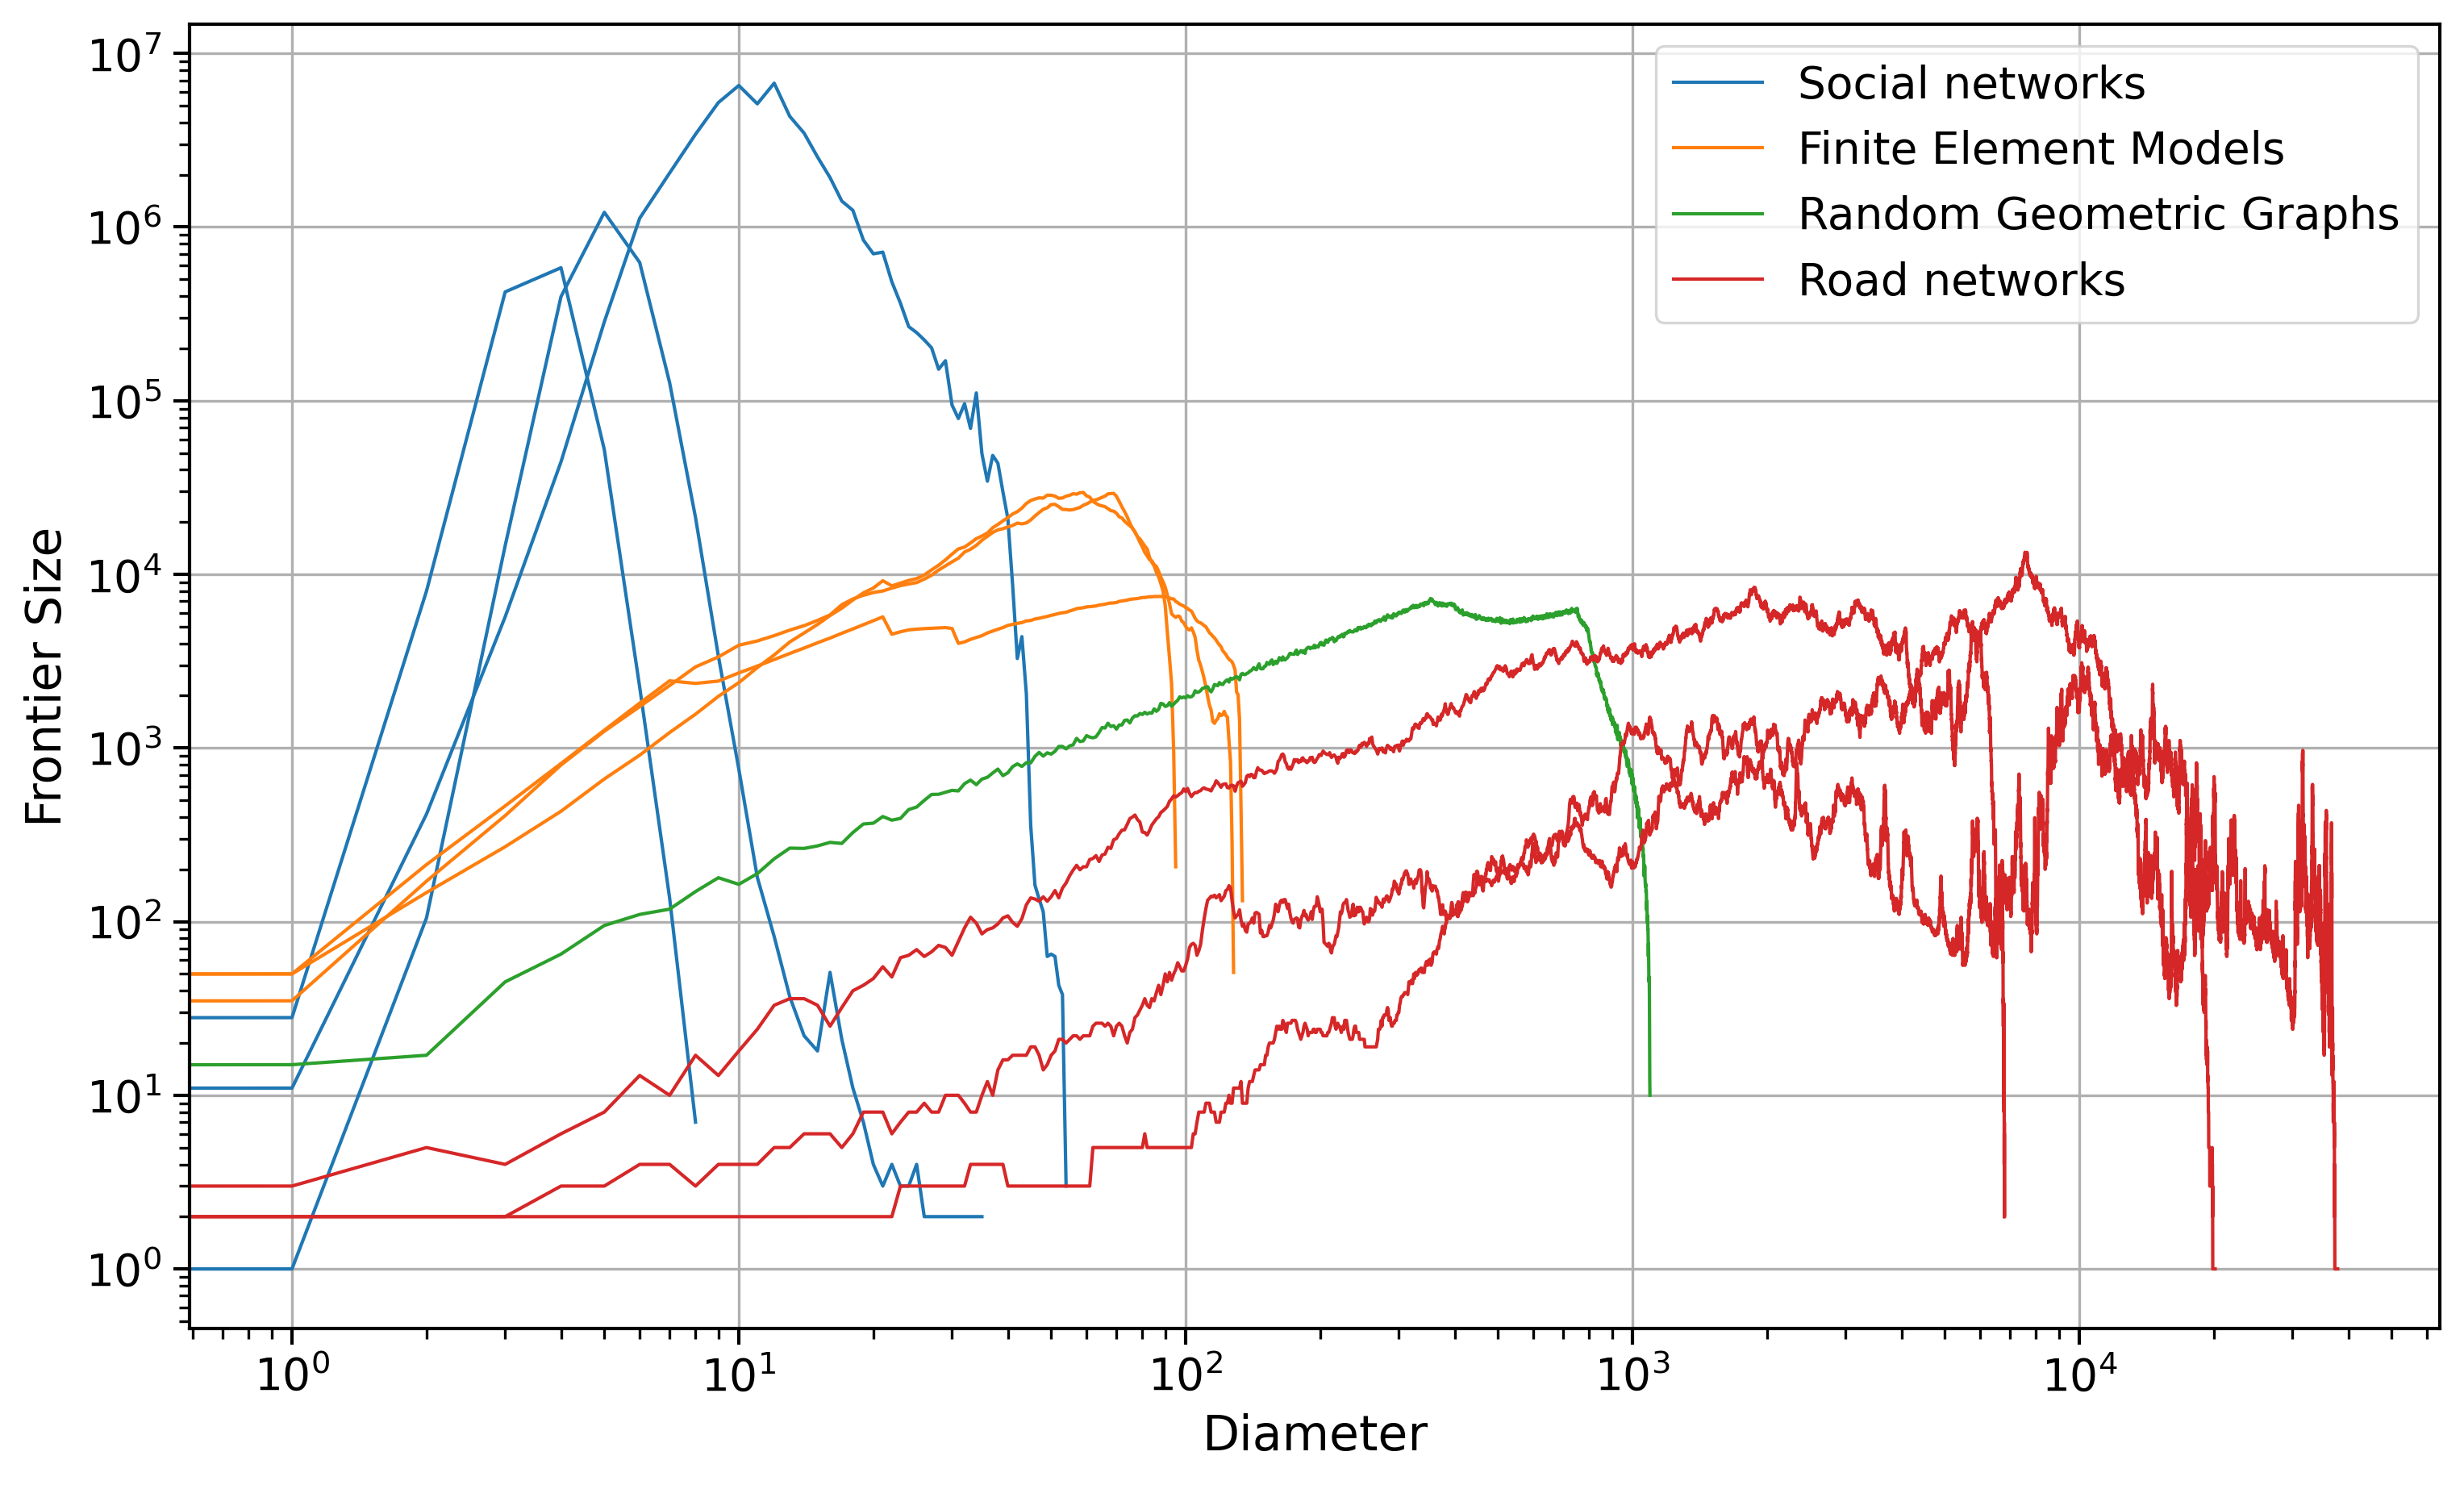
\includegraphics[width=0.8\linewidth]{images/frontiers_plot.png}
    \caption{The evolution of BFS frontier size for different graphs, colored by their graph class. The plot illustrate the frontier size at each step. Social Networks exhibit an explosive growth and subsequent collapse of the frontier, peaking at over a million vertices in fewer than 100 steps. Road Networks show a very long traversal where the frontier size remains relatively small and stable. Random Geometric Graphs display a steady expansion, confirming its large-diameter nature where the frontier never becomes excessively large. Finite Element Models exhibit intermediate behaviour, they show a more pronounced frontier growth than the road networks, representing a case where a hybrid approach might occasionally activate a Bottom-Up step.}
    \label{fig:frontiersize}
\end{figure}

\section{The Compressed Sparse Row (CSR) format}

The performance of the Top-Down and Bottom-Up traversal strategies is also dependent on the underlying data structure used to represent the graph. A widely adopted and memory-efficient format for representing sparse graphs is the Compressed Sparse Row (CSR) format. The graph's structure is encoded using two primary arrays, called \colidx{} and \rowptr{}. The \colidx{} array contains the concatenated adjacency lists of all vertices. The \rowptr{} array contains the offset of each adjacency list, where the entry at index $i$ points to the start of the $i$-th vertex's adjacency list within the \colidx{} array. The neighbors of a vertex $i$ are therefore located in the segment of the adjacency array delimited by the offsets at index $i$ and $i+1$. An example of the CSR format is shown in the top-right of \cref{fig:csr}. The space complexity of CSR is \bigO{|V| + |E|}, where $|V|$ indicates the number of vertices and $|E|$ indicates the number of edges.

Despite the algorithmic efficiency gained by this hybrid approach, the standard CSR data structure can lead to significant cache inefficiencies. During a traversal, processing a single vertex may require scattered memory accesses to separate arrays: the \rowptr{} for the CSR pointers, the \colidx{} for the neighbor lists, and algorithm-specific data like parent IDs or distances \cite{torok2020improving, andaloro2025cache}. To enhance spatial locality, the MergedCSR format was proposed by Torok \cite{torok2020improving}. This format redesigns the memory layout by merging a vertex's adjacency list into a single, contiguous data structure. By co-locating all data required to process a vertex, this layout minimizes cache misses and reduces pressure on the memory subsystem. An example of the Merged CSR layout is shown in \cref{fig:csr}. The space complexity of MergedCSR is equal to the standard CSR, i.e. \bigO{V + E}. An improvement of the original Merged CSR format is discussed in \cref{sec:mergedcsr}.

\begin{figure}[h]
    \centering
    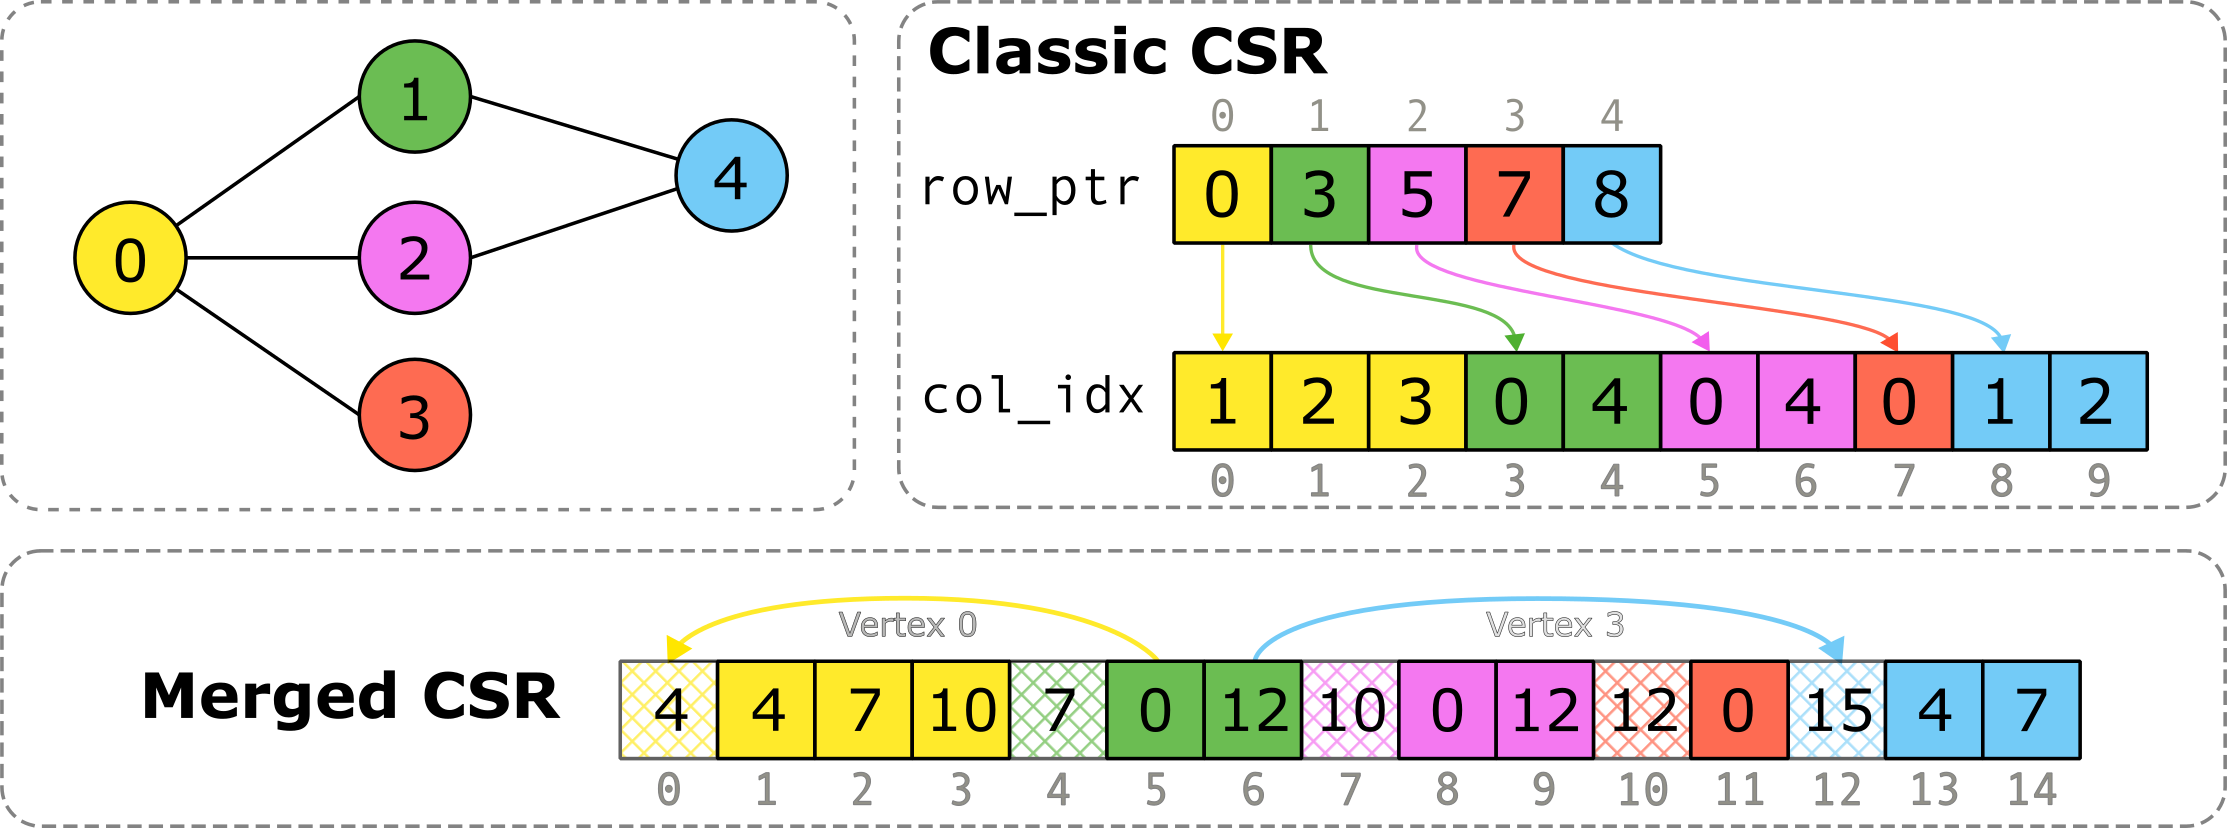
\includegraphics[width=0.8\linewidth]{images/csr.png}
    \caption{An example of the standard CSR format (top) and a cache-optimized Merged CSR layout (bottom) for the depicted graph. In the Merged CSR format, the hatched cells contain the index of the next vertex's adjacency list. Other cells contain the index of the neighboring vertex inside the Merged CSR. Arrows show the semantics of vertex 1 adjacency list, which has as neighbors vertex 0 (at location 0 in teh MergedCSR array) and vertex 4 (at location 12 in the MergedCSR array). }
    \label{fig:csr}
\end{figure}

While the CSR and MergedCSR formats provide fast retrieval of a vertex's neighbors, which is ideal for the Top-Down step, the Bottom-Up step requires also another lookup: a rapid method to check if a vertex is an element of the frontier.
This check is performed by inspecting the distances array. To facilitate this lookup, some implementations employ a bitmap to store the current frontier to improve cache utilization \cite{beamer2013direction, andaloro2025cache, arai2024doubling, niu2025berrybees}. This is because a bitmap occupies much less space than the distances array: each cell in the distance array requires 32 bits compared to only one bit in the bitmap, increasing the chances of a cache hit.

\section{Parallelization Strategies}
\label{sec:strategies}
To leverage the computational power of multicore processors, the workload of exploring each level of the graph must be distributed across multiple processing cores for concurrent execution. Due to the different structure of the Top-Down and Bottom-Up steps, the two exploration strategies are parallelized differently.

For the Top-Down step, parallelization is achieved by partitioning the current frontier among the available threads. Each thread is assigned a subset of frontier vertices and is responsible for exploring the adjacency lists of its assigned vertices. The primary challenge in this phase is managing concurrent writes to the next frontier.

In the Bottom-Up step, the source of parallelism is the complete set of vertices, which is partitioned among the threads. Each thread iterates through its the vertices in the assigned subset and checks if they are still unvisited by performing a lookup in the bitmap. If so, it checks if any of them is part of the current frontier by performing a lookup in another bitmap.

In both implementations, when multiple threads discover the same unvisited vertex simultaneously, a race condition occurs. To prevent a vertex from being added multiple times, one solution is to use atomic compare-and-swap operations to ensure only one thread successfully marks the vertex and adds it to the frontier \cite{beamer2013direction}. This approach is shown in \cref{fig:paral_shared}. Alternatively, Leiserson and Schardl observed that adding a vertex multiple times to the frontier is a benign race condition that does not affect correctness, but only performance \cite{leiserson2010work}. Their implementation therefore forgoes synchronization, accepting minor redundant work in exchange for lower overhead.

The presence of an inherently sequential data structure such as the next frontier has led to the development of alternative strategies that trade off synchronization overhead with other costs. One common solution to eliminate write contention is having each thread populate its own thread-local frontier queue \cite{beamer2013direction, leiserson2010work}. This avoids the need for atomic operations during the parallel exploration phase but introduces a subsequent merge step at the end of each level, where all thread-local queues must be consolidated into a single frontier for the next iteration. The overhead of this merge phase scales with the number of threads and the number of vertices in the frontier. This approach is shown in \cref{fig:paral_merged}.

A further optimization for the Bottom-Up steps avoids creating an explicit frontier queue by having threads update only the next frontier's bitmap \cite{andaloro2025cache}. The drawback of this `bitmap-only' approach emerges when the algorithm switches from the Top-Down to the Bottom-Up approach or vice versa. This is because the Top-Down step requires an explicit list of frontier vertices to iterate over, necessitating a full scan of the vertex set to reconstruct the frontier from the bitmap. This operation has a cost proportional to the total number of vertices. This approach is shown in \cref{fig:paral_bottomup}.

\begin{figure}[h!]
    \centering

    \begin{subfigure}[c]{0.54\textwidth}
        \centering
        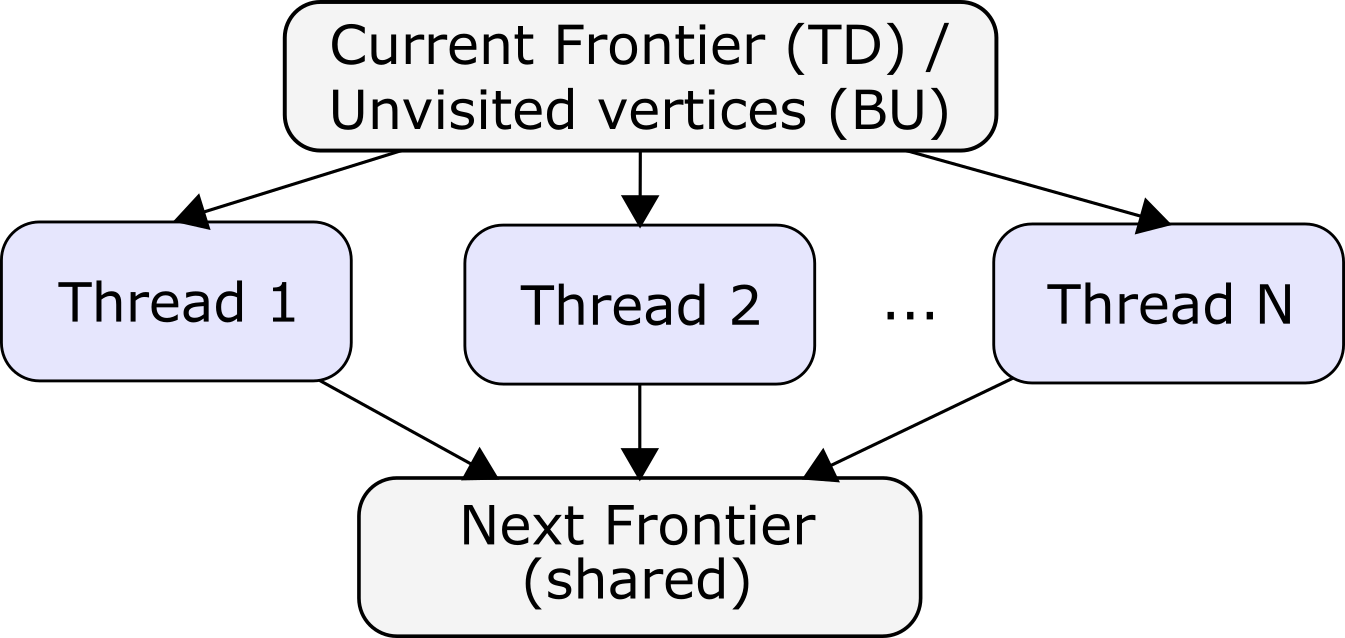
\includegraphics[width=0.8\linewidth]{images/parallelization_shared.png}
        \caption{Shared Frontier with Atomic Operations.}
        \label{fig:paral_shared}
    \end{subfigure}
    
    \vspace{0.5cm}
    
    \begin{subfigure}[c]{0.48\textwidth}
        \centering
        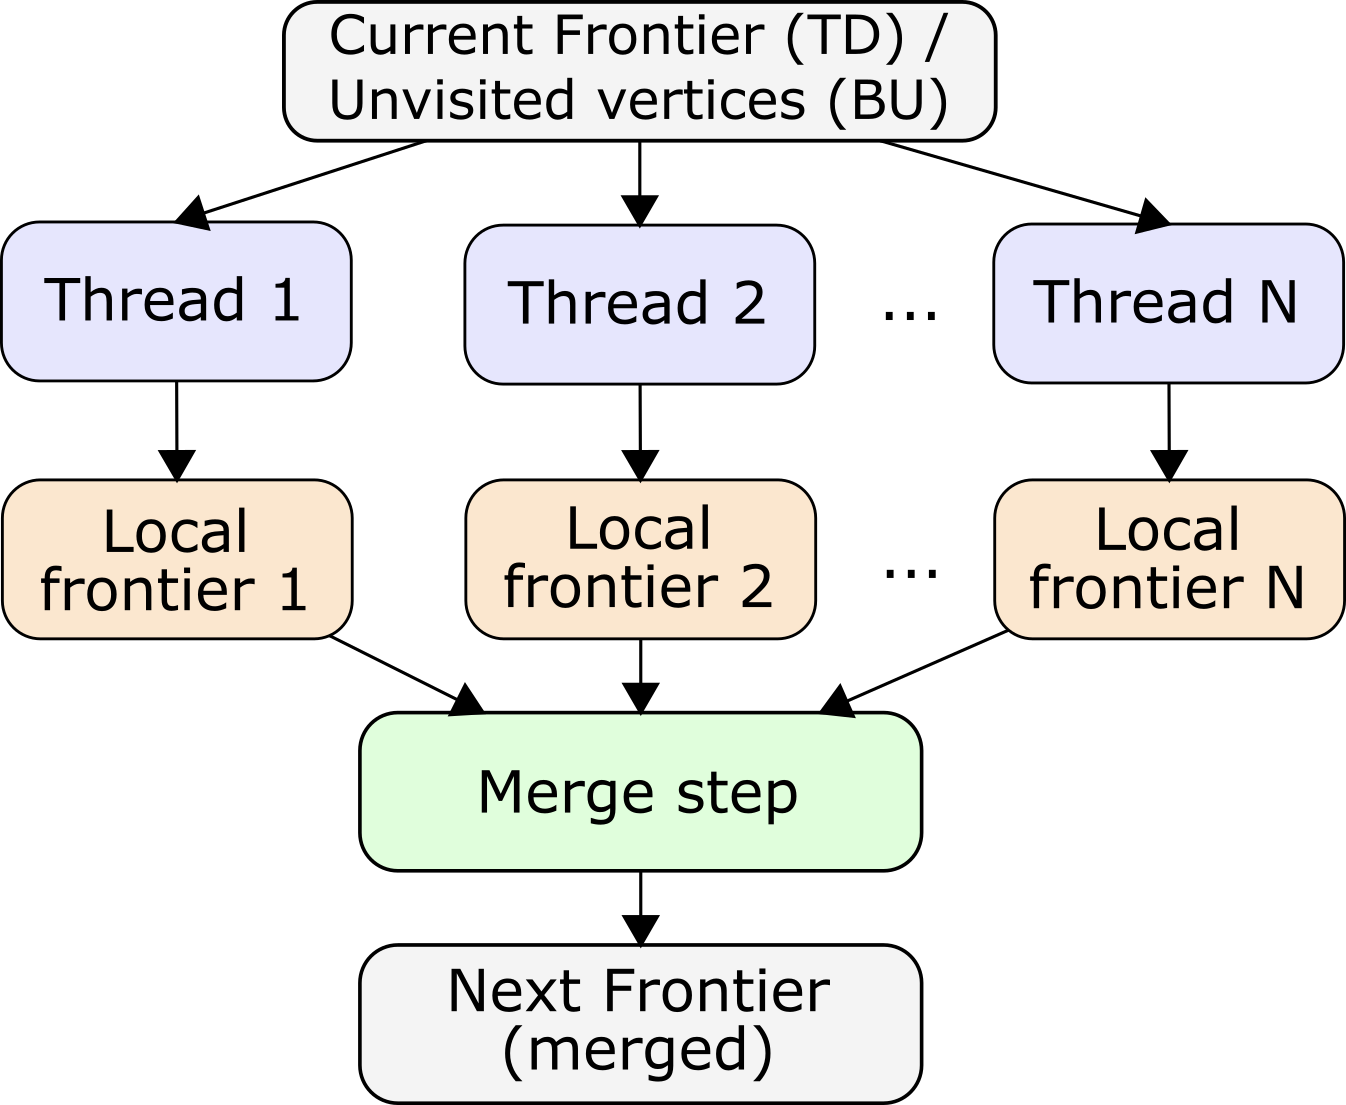
\includegraphics[width=0.8\linewidth]{images/parallelization_merged.png}
        \caption{Thread-Local Frontiers with a Final Merge Step.}
        \label{fig:paral_merged}
    \end{subfigure}
    \begin{subfigure}[c]{0.48\textwidth}
        \centering
        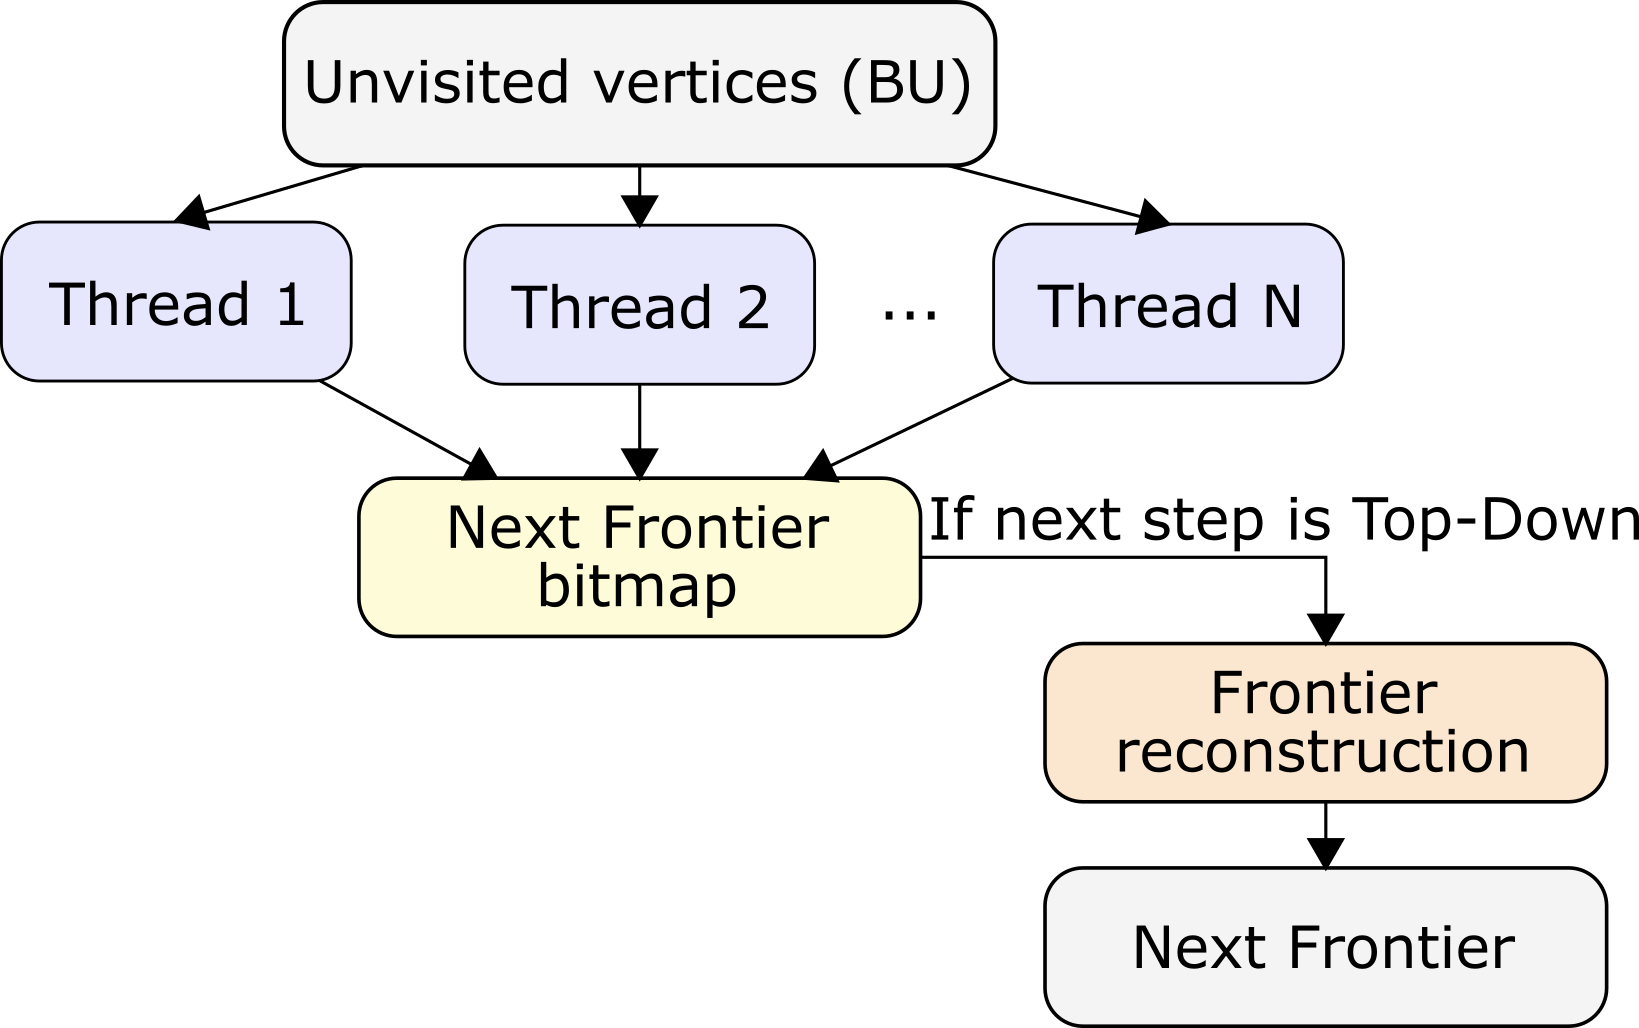
\includegraphics[width=0.9\linewidth]{images/parallelization_bottomup.png}
        \caption{Bitmap-based Approach for Bottom-Up Steps.}
        \label{fig:paral_bottomup}
    \end{subfigure}

    \caption{Proposed approaches for handling parallelization.}
    \label{fig:parallelization}
\end{figure}

\section{Performance Optimizations for Parallel BFS}
\label{sec:optimizations}
This section presents an overview of selected techniques that have been proposed for optimizing the parallel BFS algorithm.

Implementations targeting NUMA systems often employ optimizations which can be relevant also for multicore CPUs. In a NUMA system, each processor (or socket) possesses its own local memory, which offers significantly lower access latency and higher bandwidth compared to accessing memory attached to other processors via high-speed interconnects. Although the algorithms presented in \cref{cha:methodology} focus on multicore CPUs, previous research has shown that also multicore programs benefit from NUMA-like optimizations \cite{blagodurov2010case}. For example, the chiplet architecture of modern AMD EPYC processors and the segmented L3 cache of Intel Cascade Lake results in non-uniform L3 access latency, which varies based on the physical proximity of the accessing core to the cache slice containing the data \cite{velten2022memory}.

The Polymer system \cite{zhang2015numa}, which was one of the first NUMA-aware graph processing systems, co-locates vertices and connected edges within the same NUMA node as much as possible and keeps only a lightweight copy of other vertices' data, such as degree and the start index of neighboring edges. Moreover, they use a Sense-Reversal Centralized Barrier \cite{mellor1991algorithms}, which uses atomic fetch-and-add instructions to reduce contention on the software barrier between each BFS frontier expansion. As for the frontier, they use a variation of thread-local frontiers with a final merge step (as shown in \cref{fig:paral_merged}).

The optimized BFS implementation by Tithi et al. \cite{tithi2013avoiding}, instead focuses on avoiding locks and atomic instructions in shared-memory parallel BFS through optimistic parallelization. This method allows potentially conflicting operations to run in parallel, knowing that conflicts will be rare and manageable without compromising correctness. They implemented the BFS algorithm using both centralized job queues and distributed randomized work-stealing, demonstrating that lock-free versions generally outperform their lock-based counterparts. The authors also discussed strategies for optimizing their algorithms for NUMA machines, such as co-locating threads with their assigned queues on the same socket or prioritizing same-socket work-stealing targets.

Booth and Lane \cite{dennis2022adaptive}, introduced iCh, a loop scheduling method for OpenMP for irregular parallel applications on shared-memory multicore systems. Its key innovations include adaptive self-scheduling using distributed queues per thread and adaptive chunk size tuning that adjusts based on a thread's estimated iteration throughput. It also incorporates an efficient work-stealing mechanism to balance loads. These core ideas, particularly local queues and work-stealing, are directly applicable and beneficial for Breadth-First Search (BFS) implementations, which are also inherently irregular.

The ideas of Sense-Reversal Centralized
Barriers, thread-local queues, and work stealing have been implemented in a single algorithm, described in \cref{sec:pthreads}.

\section{Parallelization Frameworks}

The majority of high-performance BFS implementations for multicore CPUs utilize implicit parallelization through frameworks such as OpenMP \cite{dagum1998openmp} or Cilk++ \cite{leiserson2009cilk++}. Examples include the reference implementation for the Graph500 benchmark up to version 2.1.4 \cite{murphy2010introducing}, the direction-optimizing algorithm by Beamer \cite{beamer2013direction}, the Ligra framework \cite{shun2013ligra}, and the implementations by Tithi et al. \cite{tithi2013avoiding} and Gonzaga et al. \cite{gonzaga2024openmp}. In contrast, more comprehensive graph processing systems such as Polymer \cite{zhang2015numa} and X-Stream \cite{roy2013x} are implemented using the pthreads library\footnote{\url{https://pubs.opengroup.org/onlinepubs/7908799/xsh/pthread.h.html}}, which provides explicit thread management and synchronization. This approach is necessitated by the requirements of these systems, which support numerous graph kernels beyond BFS and often handle dynamic graph updates. Such features demand fine-grained control over memory layout, thread scheduling, and data structure synchronization, a level of control not directly offered by higher-level parallelization frameworks.

Both graph processing systems are more than 10 years old and do not include the direction-optimizing approach. It is therefore of interest to examine the performance of standalone BFS when implemented using explicit parallelization through the pthreads execution model. One such implementation, which includes also the optimizations described in \cref{sec:optimizations}, is discussed in \cref{sec:pthreads}.
  \chapter{Methodology}
\label{cha:methodology}
This chapter presents two parallel BFS implementations. \cref{sec:mergedcsr} describes a cache-optimized implementation using the MergedCSR data structure. The code is implemented in C++ using the OpenMP parallelization framework. \cref{sec:pthreads} describes an explicitly parallelized BFS implementation in C using the pthreads parallel execution model.

\section{Cache-optimized BFS using the MergedCSR data structure}
\label{sec:mergedcsr}
The performance of a Top-Down BFS traversal on a standard Compressed Sparse Row (CSR) representation is often constrained by memory latency. For each vertex explored, the algorithm must perform scattered memory accesses to three distinct data structures: the \rowptr{} array to find the offset of the adjacency list, the \colidx{} array to retrieve the neighbors, and a separate distances array to check the visited status and store the new distance. These disjoint accesses frequently lead to cache misses, as the data required to process a single vertex is not co-located in memory.

\subsection{Design and Memory Layout of MergedCSR}

To mitigate scattered memory accesses, the MergedCSR format merges the \rowptr{} and \colidx{} arrays into a single contiguous structure. The format proposed in this work extends this data structure by integrating algorithm-specific metadata directly into the graph's memory layout. In this new format, the adjacency list for each vertex is prepended with two metadata fields: the vertex's degree and its distance from the source vertex. The entire graph is thus stored in a single, large array where each vertex's data block is structured as: \texttt{[degree, distance, neighbor\_1\_idx, neighbor\_2\_idx, ...]}. Since each vertex's data block in MergedCSR is expanded by two elements (for degree and distance), the offsets for each subsequent vertex will be larger. A new \rowptr{} array is therefore necessary to correctly index into the start of each vertex's block within the new, larger structure. The space complexity for the MergedCSR array is thus \bigO{2|V| + |E|} elements. An example of the MergedCSR structure is shown in \cref{fig:improved_merged}, the pseudocode for converting from a standard CSR representation to MergedCSR is outlined in \cref{alg:convert_to_merged_csr}, and the pseudocode to extract the distances from the MergedCSR is outlined in \cref{alg:extract_distances}.

\begin{figure}
    \centering
    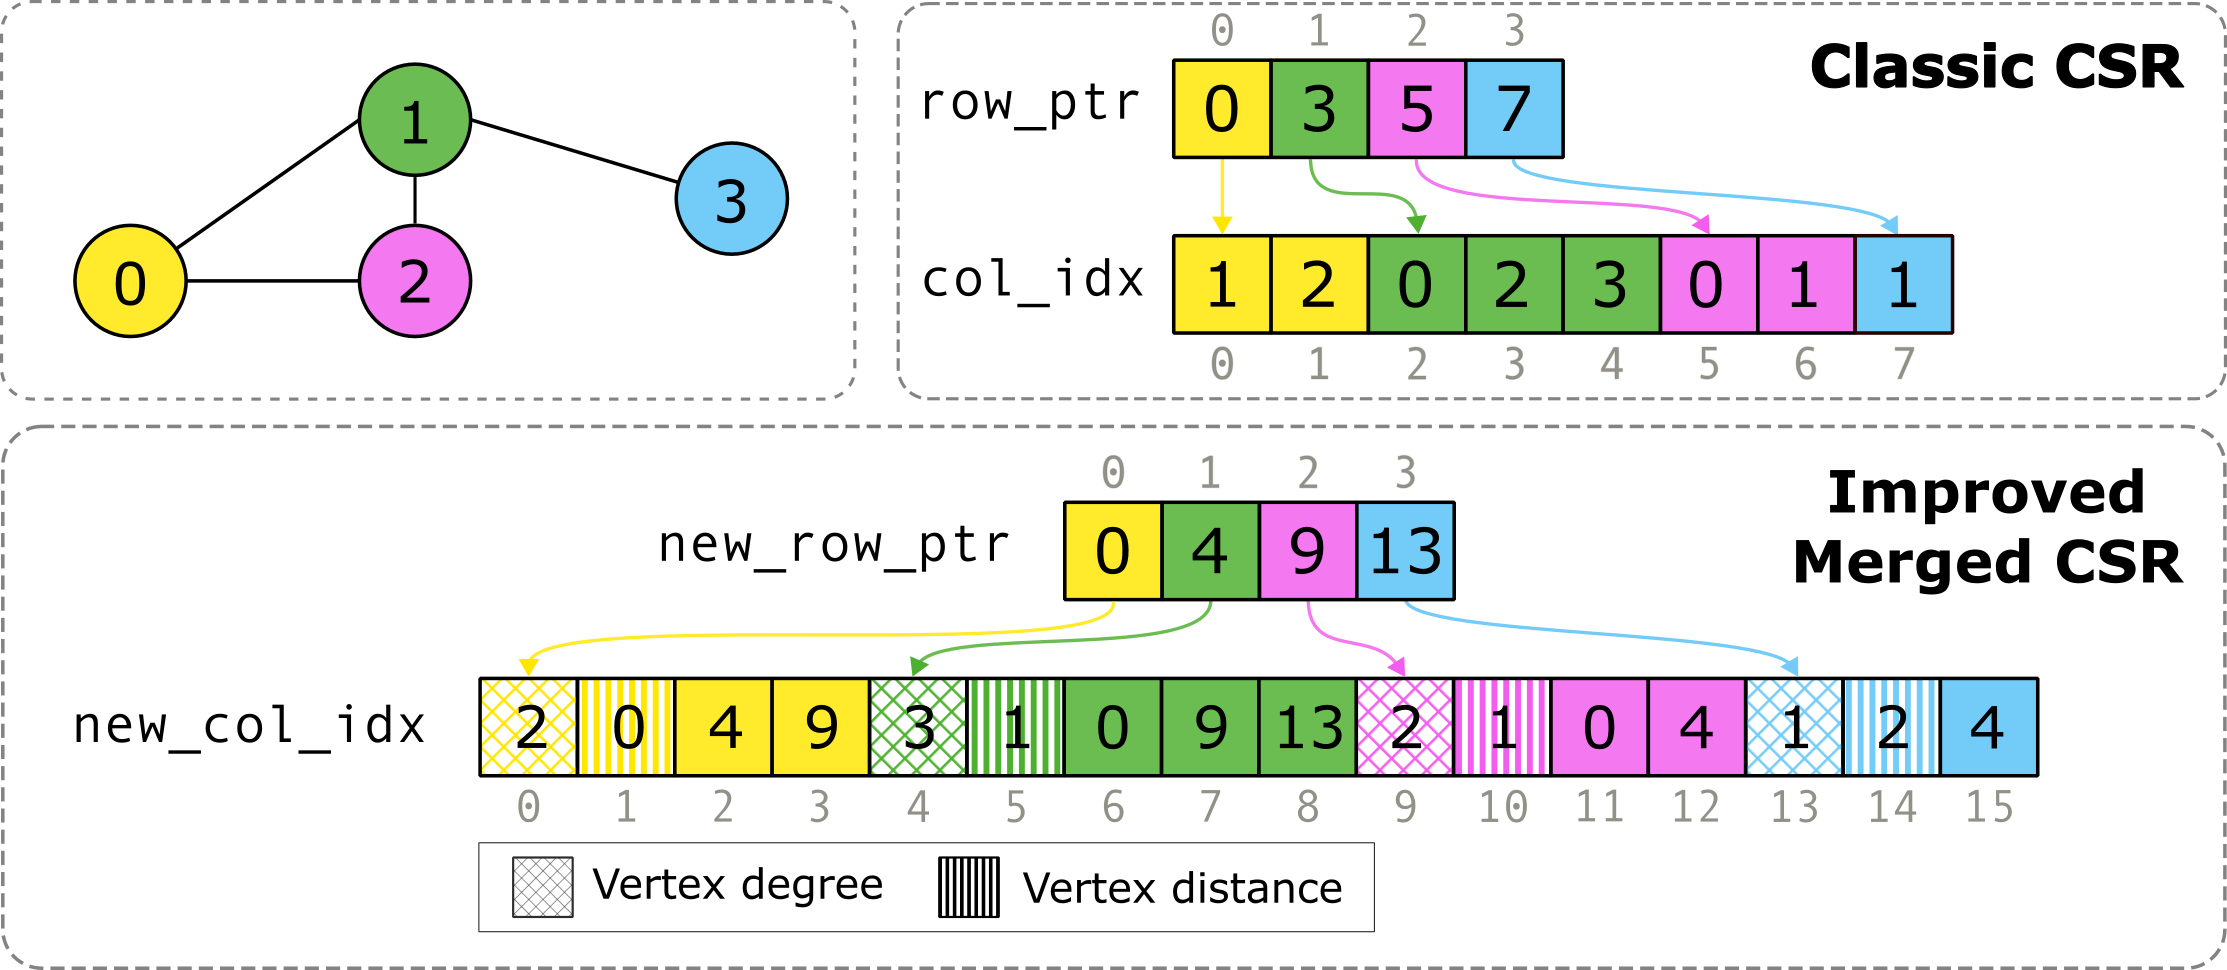
\includegraphics[width=0.8\linewidth]{images/csr_improved.png}
    \caption{An example of the improved MergedCSR structure.}
    \label{fig:improved_merged}
\end{figure}

\begin{algorithm}[H]
    % --- Define Inputs and Outputs ---
    \KwIn{
        $row\_ptr$: An array of row pointers for a standard CSR graph.\\
        $col\_idx$: An array of column indices for a standard CSR graph.\\
        $num\_vertices$: The total number of vertices in the graph.
    }
    \KwOut{
        $new\_row\_ptr$: The new row pointer array for the MergedCSR structure.\\
        $merged\_csr$: The new data structure containing degrees, distances, and neighbors.
    }
    
    \caption{Conversion to a Merged CSR Representation}
    \label{alg:convert_to_merged_csr}

    % Initialization
    $merged\_csr \gets \text{new int} [2 \times num\_vertices + |col\_idx|]$\;
    $new\_row\_ptr \gets \text{new int} [num\_vertices + 1]$\;
    $cursor \gets 0$\;

    \BlankLine % Adds a little visual space
    
    % Main loop over all vertices
    \For{$i \gets 0$ \KwTo $num\_vertices - 1$}{
        $new\_row\_ptr[i] \gets cursor$
        \tcp*{Update position of vertex $i$ in the new structure}
        \BlankLine
        $degree \gets row\_ptr[i+1] - row\_ptr[i]$\;
        $merged\_csr[cursor] \gets degree$ \tcp*{Initialize degree}
        $merged\_csr[cursor + 1] \gets \infty$ \tcp*{Initialize distance}
        $cursor \gets cursor + 2$ \tcp*{Offset cursor by number of metadata cells}

        \tcp{Copy neighbors of vertex $i$}
        \For{$j \gets row\_ptr[i]$ \KwTo $row\_ptr[i+1] - 1$}{
            \tcc{Retrieve the ID of this neighbor from the original col\_idx array}
            $neighbor\_id = col\_idx[j]$\;
            \tcc{Calculate the starting index of this neighbor's data block. Account for its original offset (row\_ptr[neighbor\_id]) plus the two metadata slots added for every vertex that comes before it (2 * neighbor\_id)}
            $new\_position \gets row\_ptr[neighbor\_id] + 2 * neighbor\_id$\; 
            \tcc{Store the calculated pointer in the new structure}
            $merged\_csr[cursor] \gets new\_position$\;
            $cursor \gets cursor + 1$ \tcp*{Advance the cursor to the next available position}
        }
    }
    $new\_row\_ptr[num\_vertices] \gets cursor$\;
    
    \BlankLine
    \KwRet{$new\_row\_ptr, merged\_csr$}\;
\end{algorithm}
\begin{algorithm}[H]
    \KwIn{
        $merged\_row\_ptr$: The row pointer array for the MergedCSR structure. \\
        $merged\_csr$: The MergedCSR data array containing metadata and neighbors. \\
        $num\_vertices$: The total number of vertices.
    }
    \KwOut{
        $distances$: An array populated with the distance of each vertex from the source.
    }
    
    \caption{Distance Extraction from MergedCSR}
    \label{alg:extract_distances}

    \BlankLine
    \For{$i \gets 0$ \KwTo $num\_vertices - 1$}{
        $offset \gets merged\_row\_ptr[i]$ \tcp*{Get start index for vertex $i$'s data block}
        $distances[i] \gets merged\_csr[offset + 1]$ \tcp*{Copy final distance from metadata}
        $merged\_csr[offset + 1] \gets \infty$ \tcp*{Reset distance in MergedCSR for next run}
    }
    \BlankLine
    
    \KwRet{$distances$}\;
\end{algorithm}

This layout is explicitly designed to exploit spatial locality. When the BFS algorithm accesses a vertex to check or update its distance, the CPU hardware will load the corresponding cache line. Because the vertex's degree and its first few neighbors are now stored immediately after the distance field, it is highly probable that this single memory fetch will also load the beginning of the vertex's adjacency list into the cache. This effectively prefetches the data required for the next frontier expansion, thereby reducing or eliminating subsequent cache misses that would have been necessary with the standard CSR format.

\subsection{Traversal Algorithm and Implementation Details}

The BFS algorithm implemented using the MergedCSR data structure is level-synchronous. This means that all vertices at a given distance $d$ from the source are fully explored before the algorithm proceeds to discover vertices at distance $d+1$.

Due to the structure of the MergedCSR, this design is optimized exclusively for the Top-Down traversal step and precludes an efficient Bottom-Up implementation. The core operation of the Bottom-Up approach involves iterating over all unvisited vertices and checking if any of their neighbors reside in the current frontier. This check is performed efficiently using a bitmap of the frontier, which requires a direct mapping from a vertex ID to its corresponding bit in the bitmap. The MergedCSR format changes the indices in the adjacency lists and breaks the index-to-vertex-ID mapping. While one could search for each neighbor's original ID to query the bitmap, the computational overhead of this \bigO{|V|} lookup would negate any performance benefits of the Bottom-Up strategy. Therefore, to maximize the benefit of the improved data locality, only the Top-Down exploration strategy is employed.

Parallelism is introduced at each level of the traversal by partitioning the vertices of the current frontier among a team of OpenMP threads. The implementation follows the ``Thread-Local Frontiers'' with a ``Final Merge Step'' parallelization strategy (see \cref{sec:strategies} and \cref{fig:paral_merged}). This strategy is realized efficiently through a custom OpenMP reduction. Instead of having all threads contend for locks or use atomic operations to write to a single shared next-frontier, each thread populates its own private, thread-local version of the next frontier. At the end of the parallel exploration for that level, OpenMP automatically performs a final merge step to combine all the thread-local frontiers into a single, unified frontier for the next iteration.
\begin{minted}{cpp}
#pragma omp declare reduction(vec_add \
    : frontier : omp_out.insert(omp_out.end(), omp_in.begin(), omp_in.end()))
\end{minted}
This custom reduction instructs OpenMP on how to combine the thread-local frontiers at the end of the parallel loop: the contents of each thread's private frontier (\texttt{omp\_in}) are appended to the master frontier (\texttt{omp\_out}). This direct vector concatenation avoids the need for manual synchronization. The custom reduction is then applied to the for loop that iterates over the vertices in the frontier, as shown the the following listing.
\begin{minted}[xleftmargin=20pt, breaklines, linenos]{cpp}
#pragma omp parallel for reduction(vec_add : next_frontier) schedule(static) if (this_frontier.size() > 50)
for (const auto &v : this_frontier) {
  eidType end = v + 2 + DEGREE(v);
  // Iterate over neighbors
  for (eidType i = v + 2; i < end; i++) {
      eidType neighbor = merged_csr[i];
      // If neighbor is not visited, add to frontier
      if (DISTANCE(neighbor) == std::numeric_limits<weight_type>::max()) {
        if (DEGREE(neighbor) != 1) {
          next_frontier.push_back(neighbor);
        }
        // Set the neighbor's distance
        DISTANCE(neighbor) = distance;
      }
  }
}
\end{minted}

The outer loop is parallelized using the \texttt{schedule(static)} clause, which pre-allocates fixed-size chunks of the frontier to each thread. While graph traversal workloads are inherently irregular and can lead to load imbalance, empirical evaluation demonstrated that the low overhead of static scheduling consistently outperformed the more complex dynamic scheduling strategies offered by OpenMP.

Furthermore, parallelization is enabled only when the frontier size exceeds a threshold of 50 vertices. This optimization prevents the runtime overhead associated with creating and managing the thread team from outweighing the computational speedup on small workloads, for which sequential execution is faster.

\subsection{Postprocessing and Generality}

Once the BFS traversal is complete, the distance values are embedded within the MergedCSR structure. A final postprocessing step is required to extract these values into a standard distances array. This is accomplished with a simple parallel loop that iterates from $0$ to $|V|-1$, using the updated \rowptr{} to locate the distance field for each vertex and copy its value. The pseudocode of this procedure is outlined in \cref{alg:extract_distances}.

The same framework can be adapted to produce a parent array instead of a distance array. In this variation, the distance field in the MergedCSR structure is repurposed to store the parent ID of each vertex. The logic of the traversal remains largely the same, with the algorithm storing the ID of the discovering vertex instead of the new distance level.

\newpage

\section{Case study: Explicit parallelization of BFS using pthreads}
\label{sec:pthreads}

This section presents an alternative BFS implementation that avoids high-level parallelization frameworks and instead uses explicit thread management with the POSIX Threads (pthreads) library in C. This approach provides fine-grained control over thread lifecycle, work distribution, and synchronization. The design is built upon three core components: a persistent thread pool to minimize thread creation overhead, a chunk-based frontier with a work-stealing mechanism to dynamically balance the load, and a low-overhead, centralized barrier to ensure level-synchronous traversal. For its underlying graph representation, this implementation utilizes the cache-optimized Merged CSR data structure.

\subsection{The Chunk-Based Frontier}

The parallel frontier is managed by a set of data structures designed to minimize lock contention, reduce dynamic memory allocation overhead, and facilitate a dynamic work-stealing load balancing strategy. The design is composed of three primary structures: the \texttt{Chunk}, the \texttt{ThreadChunks} queue, and the top-level \texttt{Frontier} container. A schematic representation of the combined structures is shown in \cref{fig:frontier}.

\paragraph{The \texttt{Chunk} structure} This structure represents the atomic unit of work distributed among threads. The structure consists of a fixed-size block containing an array of vertex identifiers. The \texttt{CHUNK\_SIZE} constant defines the capacity of each block. This design choice amortizes the overhead associated with managing the frontier; instead of threads manipulating individual vertices in a shared queue, they acquire and process entire blocks of work at a time. The \texttt{next\_free\_index} field serves as a stack pointer, allowing the \texttt{Chunk} object to function as a Last-In, First-Out (LIFO) buffer. Vertices are pushed by placing them at this index and incrementing it, and popped by decrementing the index. When \texttt{next\_free\_index} is zero, the chunk is empty. This LIFO access pattern is cache efficient, as vertices that were just written to the chunk are also the first ones to be read and processed.

\begin{minted}{c}
typedef struct {
  ver_t vertices[CHUNK_SIZE];
  int next_free_index;
} Chunk;
\end{minted}

\paragraph{The \texttt{ThreadChunks} structure} This structure manages a dynamic array of pointers to a set of \texttt{Chunk} structures. The \texttt{top\_chunk} index makes the array function as a stack, while the \texttt{chunks\_size} field tracks the total allocated capacity of this array. If a thread's queue runs out of space (i.e., \texttt{top\_chunk} reaches \texttt{chunks\_size}), the chunks array is reallocated to double its previous capacity. This expansion strategy, which is implemented using the \texttt{realloc()} function, ensures that the cost of adding new chunks has amortized cost \bigO{1}. Similarly to the \texttt{Chunk} structure, this structure also acts as a LIFO stack to exploit temporal cache locality. During the frontier expansion phase of a BFS level, a thread creates and populates new chunks with newly discovered vertices. In the subsequent BFS level, the thread will pop the chunks to process them. Because the top chunks were the last to be inserted, they also have a higher probability of still residing in the thread's private L1 or L2 caches, therefore optimizing the cache usage. Each \texttt{ThreadChunks} structure contains also its own \texttt{pthread\_mutex\_t} lock. A thread must acquire this lock to add or remove a \texttt{Chunk} from its own queue. This same lock must be acquired also by any other thread attempting to "steal" a Chunk from this queue.

\begin{minted}{c}
typedef struct {
  Chunk **chunks;
  int chunks_size;
  int top_chunk;
  pthread_mutex_t lock;
} ThreadChunks;
\end{minted}

\paragraph{The \texttt{Frontier} structure} This structure consists of an array of pointers to \texttt{ThreadChunks} objects, providing a centralized point of access to each thread's individual work queue. This allows a work-stealing thread to iterate through all other threads and attempt to acquire work from their respective queues. The \texttt{Frontier} structure contains also a \texttt{thread\_chunk\_counts} array, which stores the number of active chunks per thread. This array provides a fast, lock-free snapshot of the entire system's work distribution. An idle thread can scan this array to quickly identify the busy threads and steal work from them, without incurring the high contention cost of acquiring each thread's mutex simply to inspect its queue size.

\begin{minted}{c}
typedef struct {
  ThreadChunks **thread_chunks;
  int *thread_chunk_counts;
} Frontier;
\end{minted}

\begin{figure}[h]
    \centering
    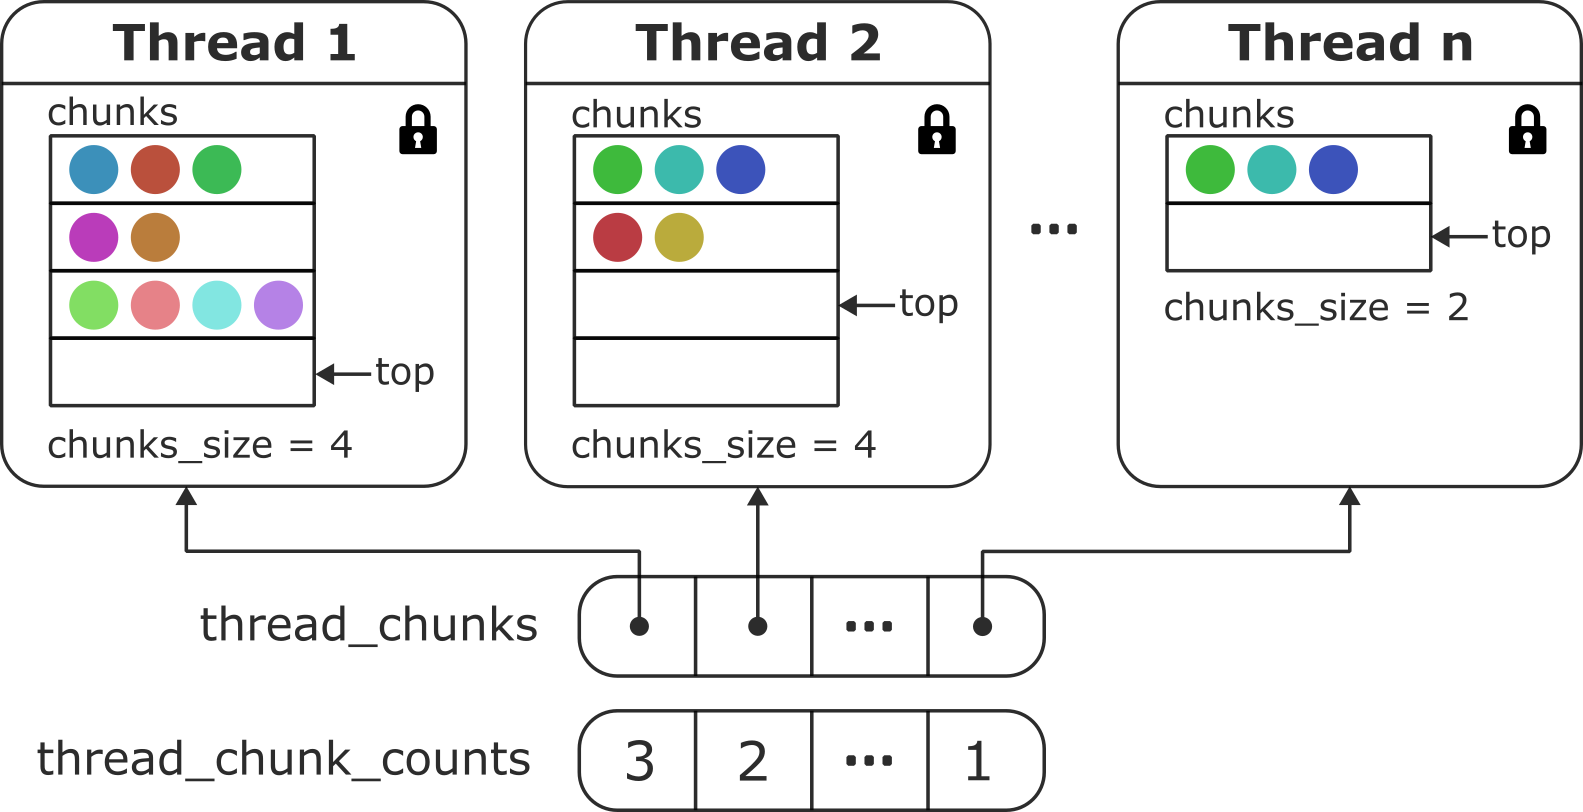
\includegraphics[width=0.7\linewidth]{images/frontier.png}
    \caption{An overview of the \texttt{Frontier} data structure for parallel BFS. The top-level \texttt{Frontier} structure contains pointers to each thread's private \texttt{ThreadChunks} work queue. Each \texttt{ThreadChunks} contains a stack of \texttt{Chunks}, with the top pointer indicating the next available slot in the stack. The colored circles represent the vertices contained in each chunk. Access to the \texttt{chunks} array is serialized by a dedicated mutex (represented by the lock icon). The auxiliary \texttt{thread\_chunk\_counts} array provides lock-free access to the number of chunks of each thread.}
    \label{fig:frontier}
\end{figure}

\subsection{Dynamic Load Balancing via Work-Stealing}

To counteract the inherent workload imbalance characteristic of irregular graph traversal, a dynamic work-stealing mechanism is implemented. This protocol allows idle threads to acquire work from busy threads.

A thread transitions from a "worker" to a "thief" state as soon as it has processed all the chunks in its own \texttt{ThreadChunks} queue. Once its own work queue is empty, it initiates the work-stealing protocol. First, the stealing thread iterates through the \texttt{thread\_chunk\_counts} array, looking for any thread whose chunk count is greater than one. This heuristic prevents excessive lock contention, particularly during phases of the BFS where the frontier is small. If the entire frontier consists of only a single chunk, this rule prevents all but one thread from repeatedly attempting to lock the same mutex, a phenomenon which would serialize execution and negate the benefits of parallelism.

Upon identifying a potential victim that satisfies this condition, the thief proceeds to attempt a steal. It first tries to acquire the victim thread's \texttt{pthread\_mutex\_t} lock. Once the lock is successfully acquired, the thief performs a second check on the victim's chunk count. This check is necessary to prevent a race condition; it is possible that another thief stole a chunk in the time between the initial lock-free check and the successful acquisition of the lock. If the victim thread still has more than one chunk available, the steal is executed. The thief decrements the victim's \texttt{top\_chunk} index to claim a chunk, and the corresponding value in the shared \texttt{thread\_chunk\_counts} array to ensure the global view of work distribution remains consistent. After these modifications, the thief releases the victim's lock and begins processing the vertices within the stolen chunk.

Upon finishing the stolen chunk, the thief thread re-initiates the work-stealing protocol, starting a new scan of the \texttt{thread\_chunk\_counts} array to find another victim. This loop continues until the thread performs a full scan of the \texttt{thread\_chunk\_counts} array and finds that all entries are zero. This state signifies that the entire frontier for the current level has been processed. At this point, the thread stop its execution for the current level and proceed to the synchronization barrier. The flowchart of the work-stealing protocol is shown in \cref{fig:workstealing}.

\begin{figure}[h]
    \centering
    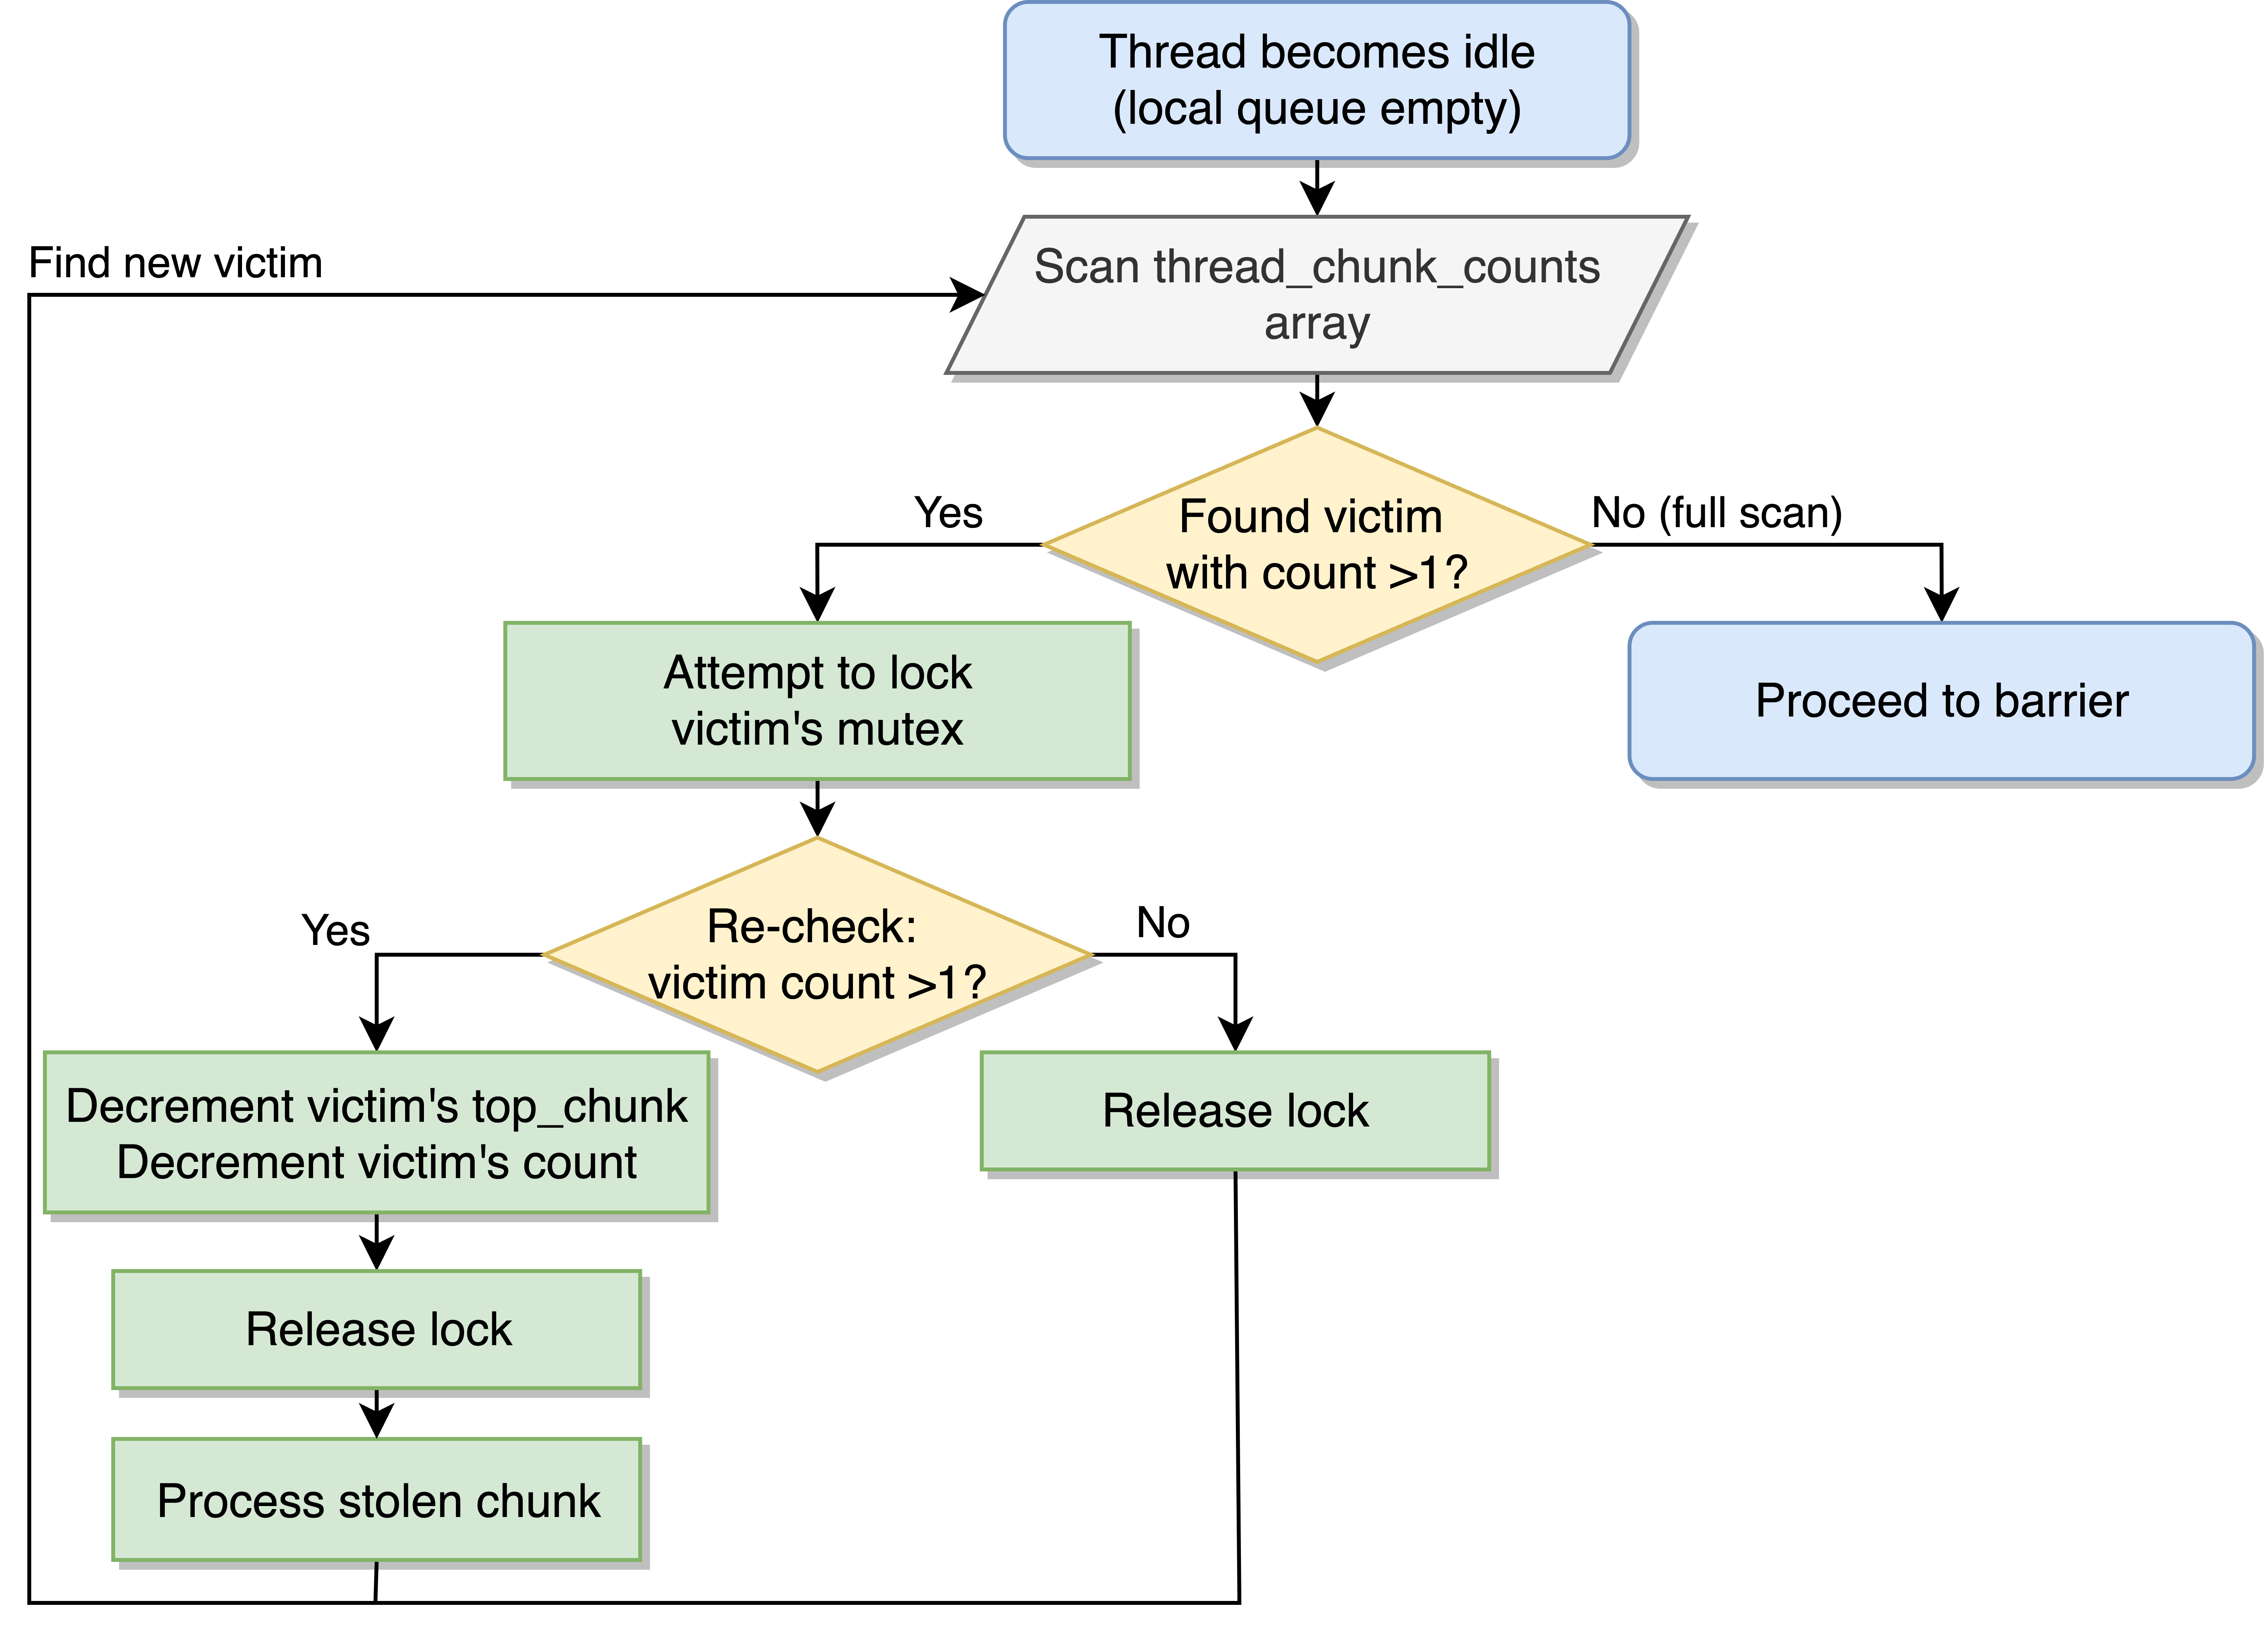
\includegraphics[width=0.7\linewidth]{images/workstealing.png}
    \caption{The work-stealing protocol.}
    \label{fig:workstealing}
\end{figure}

\subsection{Thread Pool and Work Dispatch}

The explicit parallelization of the BFS algorithm is built upon a persistent thread pool. This design is motivated by the high performance cost associated with the creation and destruction of operating system threads. By creating a fixed-size pool of worker threads once at program initialization and reusing them for each subsequent BFS traversal, the significant overhead of thread management is amortized all BFS runs. The \texttt{thread\_pool\_t} structure serves as the central control block for the entire pool, managing thread handles, state, and the synchronization primitives required for coordination between the main (parent) thread and the worker (child) threads.

\begin{minted}{c}
typedef struct {
  pthread_cond_t cond_children;    // Used to signal child threads
  pthread_mutex_t mutex_children;
  pthread_cond_t cond_parent;      // Used to signal the parent thread
  pthread_mutex_t mutex_parent;
  
  pthread_t threads[MAX_THREADS];  // Set of spawned threads
  int thread_ids[MAX_THREADS];     // Set of spawned threads' IDs
  atomic_uint run_id;              // Counter for work cycles
  atomic_bool stop_threads;        // Flag to signal threads to terminate
  atomic_bool children_done;       // Flag to signal parent that workers are done
  
  void *(*routine)(void *);        // Stores the worker function pointer
} thread_pool_t;
\end{minted}

\paragraph{Synchronization Primitives} The implementation employs two distinct pairs of mutexes and condition variables to manage the two-way communication between the main thread and the worker threads. The \texttt{cond\_children} condition variable and its associated \texttt{mutex\_children} are used exclusively to manage the state of the worker threads. The main thread signals \texttt{cond\_children} to wake the workers and dispatch a new work cycle. Symmetrically, the \texttt{cond\_parent} condition variable and \texttt{mutex\_parent} are used by the main thread. This allows it to enter an efficient wait state, blocking on \texttt{cond\_parent} until a worker signals that the entire BFS task is complete. This separation makes the synchronization logic simple, preventing potential deadlocks or race conditions that could arise from using a single set of primitives for bidirectional communication.

\paragraph{State and Signaling Variables} The coordination between threads is orchestrated through a set of atomic state variables that ensure thread-safe communication without requiring locks for every state change. The primary signaling mechanism is the atomic \texttt{run\_id} integer, which functions as a work cycle counter. Using a counter instead of a simple boolean flag provides a more robust design, as each work dispatch is identified by a unique ID. This prevents workers from accidentally performing a work cycle multiple times in the case of a spurious wakeup, as they explicitly check their local counter against the global one. The \texttt{stop\_threads} atomic boolean variable is used to signal a graceful shutdown of the pool. Finally, the \texttt{children\_done} atomic boolean variable is used to signal that the children have terminated the BFS.

\paragraph{Thread pinning} Upon creation, each thread is pinned to a specific CPU core using the Linux-specific \texttt{pthread\_setaffinity\_np} function. This overrides the default behavior of the operating system's scheduler, which may otherwise migrate threads between cores to balance the overall system load. The primary benefit of this is the enhancement of data locality. As a thread executes, it populates its core's private L1 and L2 caches with frequently accessed data, such as its stack and the graph data from its assigned work chunks. If the thread were to be migrated, these warm caches would be lost, and it would have to repopulate the cold caches of the new core, incurring significant latency from fetching data from the L3 cache or main memory \cite{gandham2024occ}.

\vspace{0.5em}
\subsubsection{Synchronization Lifecycle} \label{sec:synchronization}
The interaction between the main thread and the worker threads follows a specific order which ensures minimal busy-waiting and efficient CPU usage through the use of condition variables. The state diagram of the main and worker threads is shown in \cref{fig:synchronization}.

\paragraph{Initialization and Creation} The pool is first initialized with \texttt{init\_thread\_pool()}, which sets up the mutexes and condition variables. Subsequently, \texttt{thread\_pool\_create()} spawns \texttt{MAX\_THREADS} worker threads. Each thread is assigned a unique ID and it immediately enters a wait state. In this state, each worker thread acquires the children's mutex and enters a while loop that blocks on the \texttt{cond\_children} condition variable. A worker is only released from this wait when the global \texttt{run\_id} (controlled by the main thread) is equal to or greater than the worker's own local \texttt{run\_id}. Upon waking, the worker increments its local \texttt{run\_id}, effectively "consuming" the work signal, which prepares it to wait for the next cycle after its current task is complete.

\paragraph{Work Dispatch} The main thread initiates a BFS traversal by calling \texttt{thread\_pool\_start\_wait()}. This function acts as the dispatcher. It first acquires the necessary locks, then increments the global \texttt{run\_id}, and finally calls \texttt{pthread\_cond\_broadcast()}. This broadcast wakes up all waiting worker threads simultaneously, causing them to exit their wait state and begin executing the main BFS routine.

\paragraph{Completion and Notification} After dispatching the work, the main thread immediately blocks by calling \texttt{pthread\_cond\_wait()} on the parent's condition variable, \texttt{cond\_parent}. It remains in this sleep state, consuming no CPU cycles, until the entire BFS traversal is complete. The last worker thread to finish the final step of the BFS is responsible for calling \texttt{thread\_pool\_notify\_parent()}. This function sets the \texttt{children\_done} predicate to true and signals \texttt{cond\_parent}, waking the main thread and allowing the program to proceed.

\paragraph{Termination} To shut down the pool, the main thread calls \texttt{thread\_pool\_terminate()}. This function sets the \texttt{stop\_threads} flag to true and broadcasts one final signal on the \texttt{cond\_children} condition variable to ensure any sleeping threads wake up. The awakened threads check the \texttt{stop\_threads} flag and call \texttt{pthread\_exit} to terminate gracefully. The main thread then calls \texttt{pthread\_join} on all worker threads to guarantee they have all exited before the program's resources are deallocated.

\begin{figure}
    \centering
    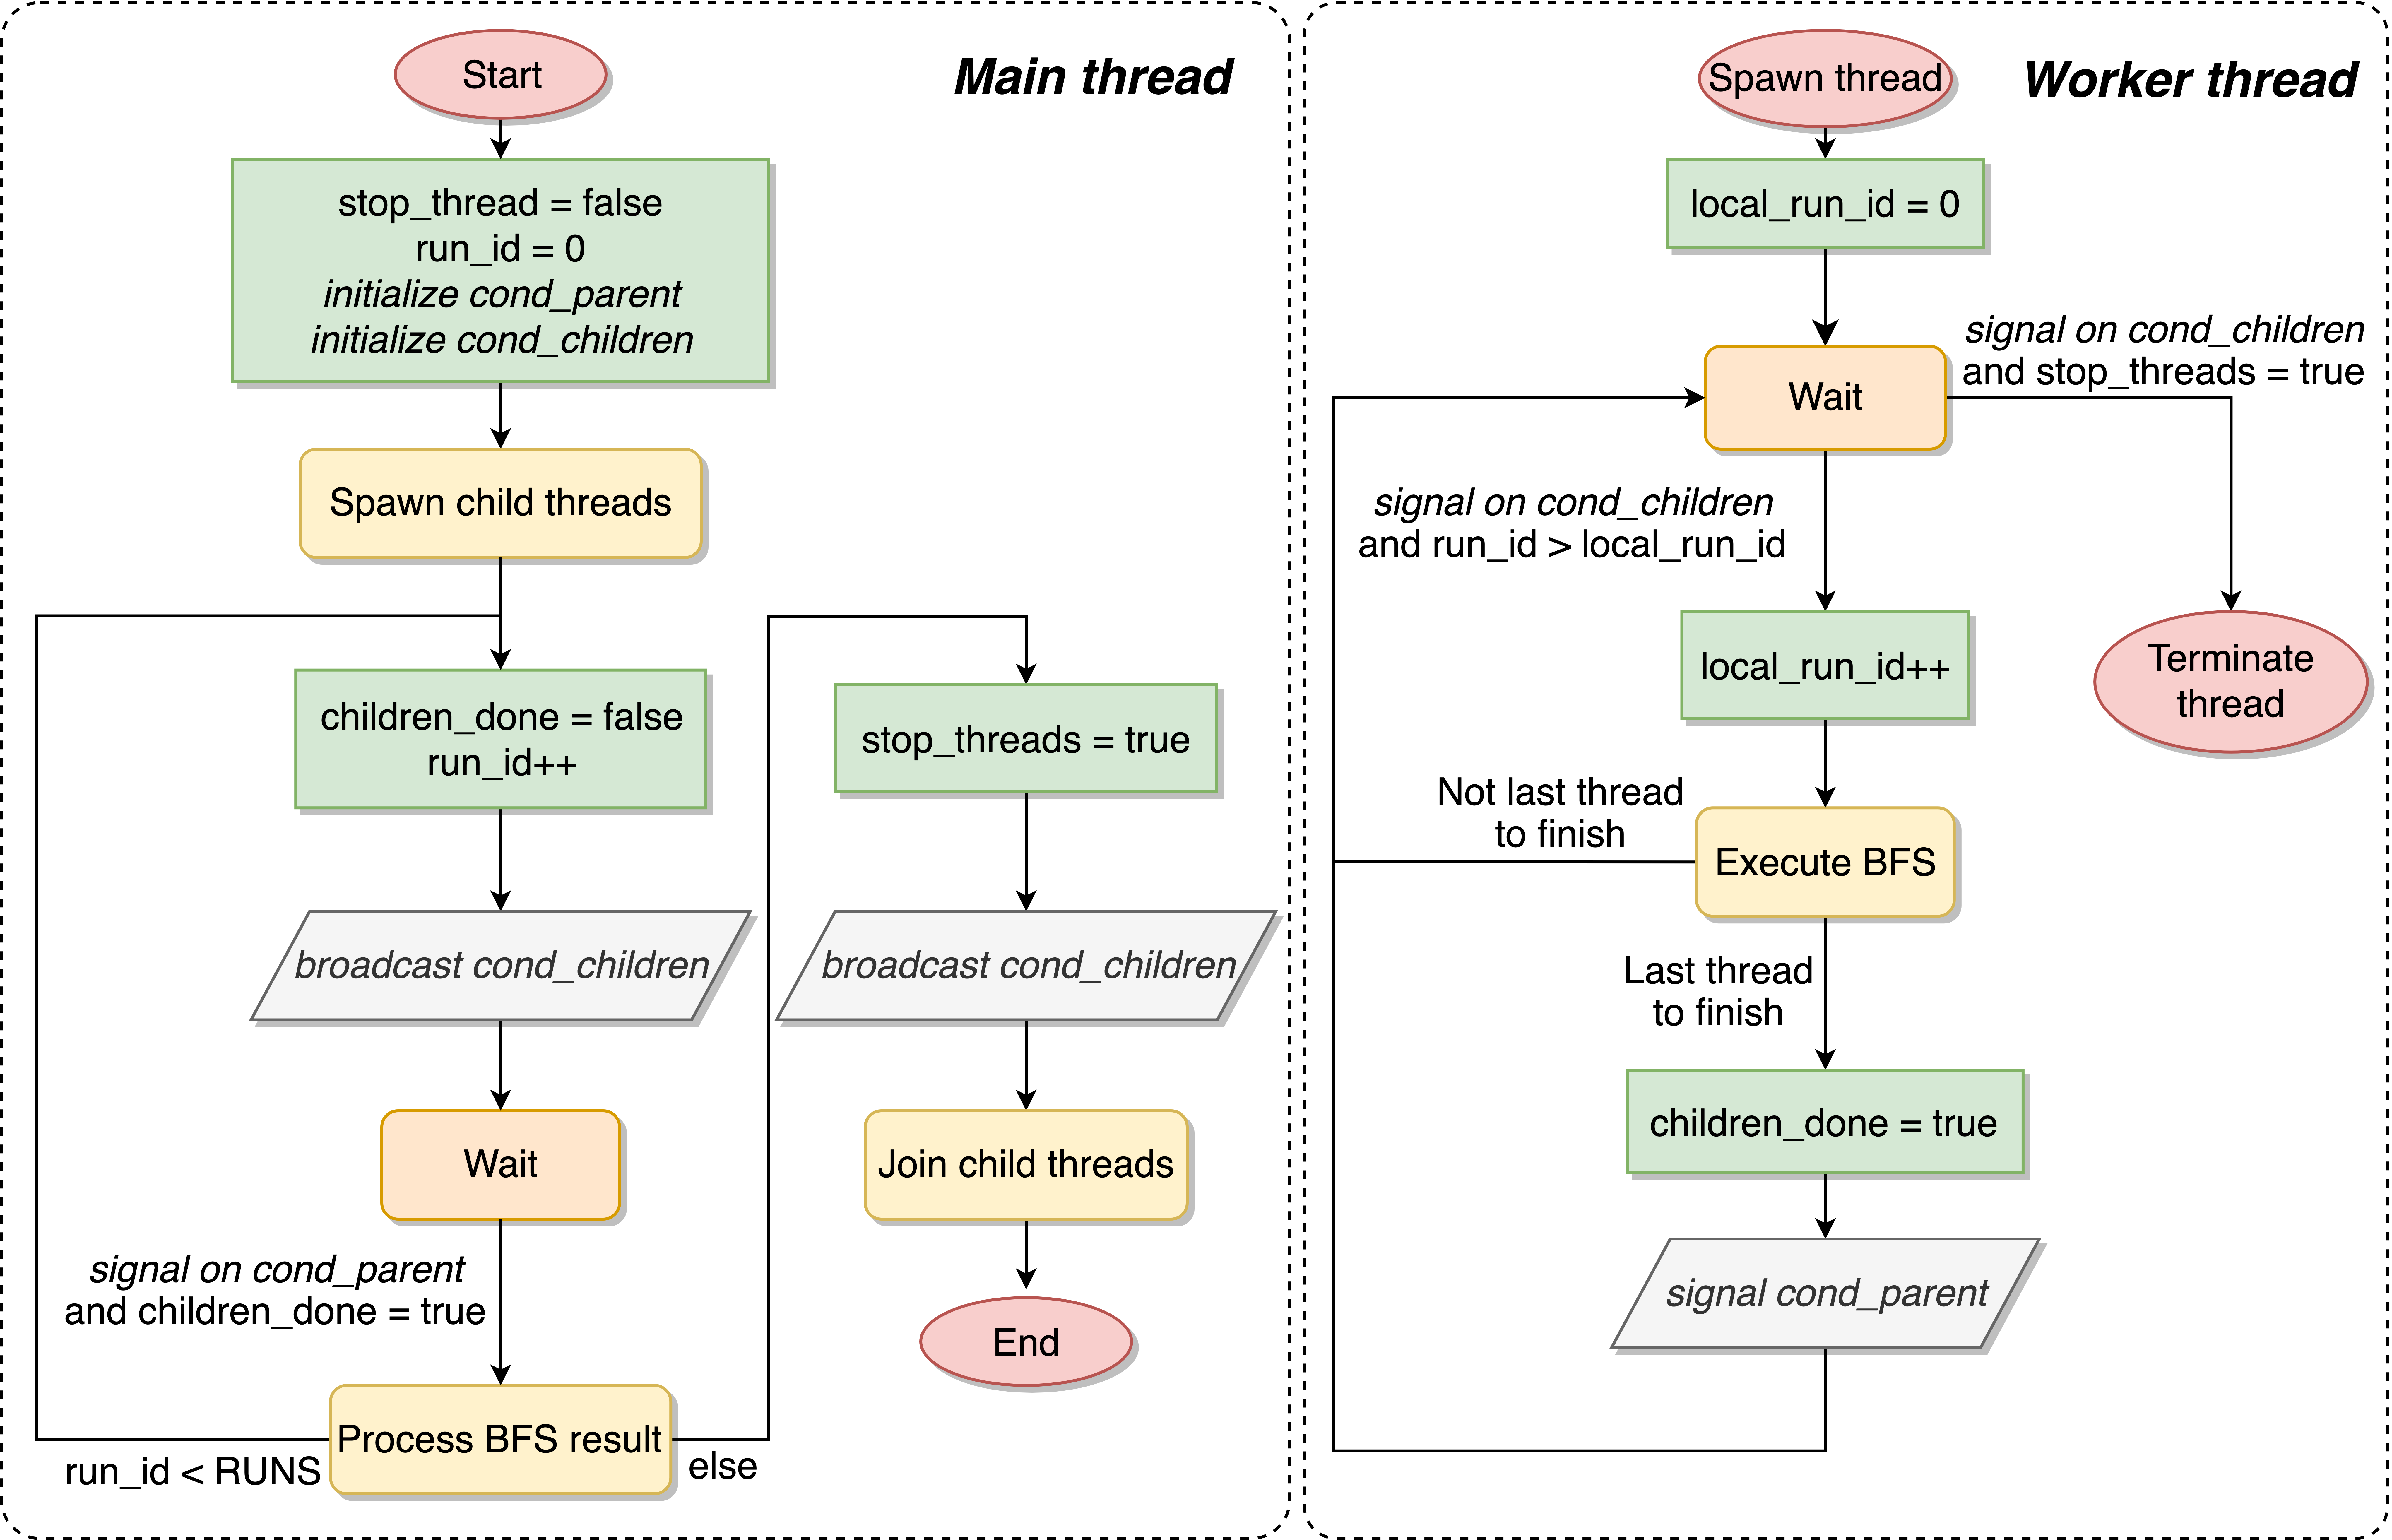
\includegraphics[width=0.9\linewidth]{images/threads.png}
    \caption{State diagrams of the main and worker threads. The \texttt{RUNS} variable contains the total number of iterations of the BFS.}
    \label{fig:synchronization}
\end{figure}

\subsection{Level Synchronization and Barrier Implementation}

The level-synchronous BFS requires a barrier, which ensures all threads have completed their work for the current level before any thread begins processing the next. This implementation uses a custom barrier that is a variation of the Sense-Reversal Centralized Barrier.

The synchronization is managed using an atomic counter, \texttt{active\_threads}, and the \texttt{distance} variable. At the beginning of each level, \texttt{active\_threads} is reset to \texttt{MAX\_THREADS}. When a thread finishes processing all of its work for the current level (including any stolen work), it atomically decrements this counter.

The last thread to finish its work is designated the "leader" for that level. The thread notices that it is the leader because the \texttt{active\_threads} variable is equal to one when it arrives at the barrier. This leader thread is responsible for performing the serial tasks required between levels: swapping the pointers for the current and next frontiers, checking if the new frontier is empty to determine if the entire BFS should terminate, and finally, incrementing the global \texttt{distance} variable. If there are no vertices left in the frontier, instead of incrementing the global \texttt{distance} variable, it sets the \texttt{exploration\_done} boolean variable and notifies the main thread that the BFS has terminated (as explained in \cref{sec:synchronization}).

The other, non-leader threads, after decrementing the counter, enter a spin-wait loop, continuously checking if the distance has been incremented by the leader. The act of incrementing distance serves as the "sense-reversal" signal, releasing all waiting threads from the barrier simultaneously to begin work on the next level. This design avoids the overhead associated with \texttt{pthread\_barrier\_t} objects as it relies on a single atomic counter and a shared variable for coordination.

\begin{figure}[H]
    \centering
    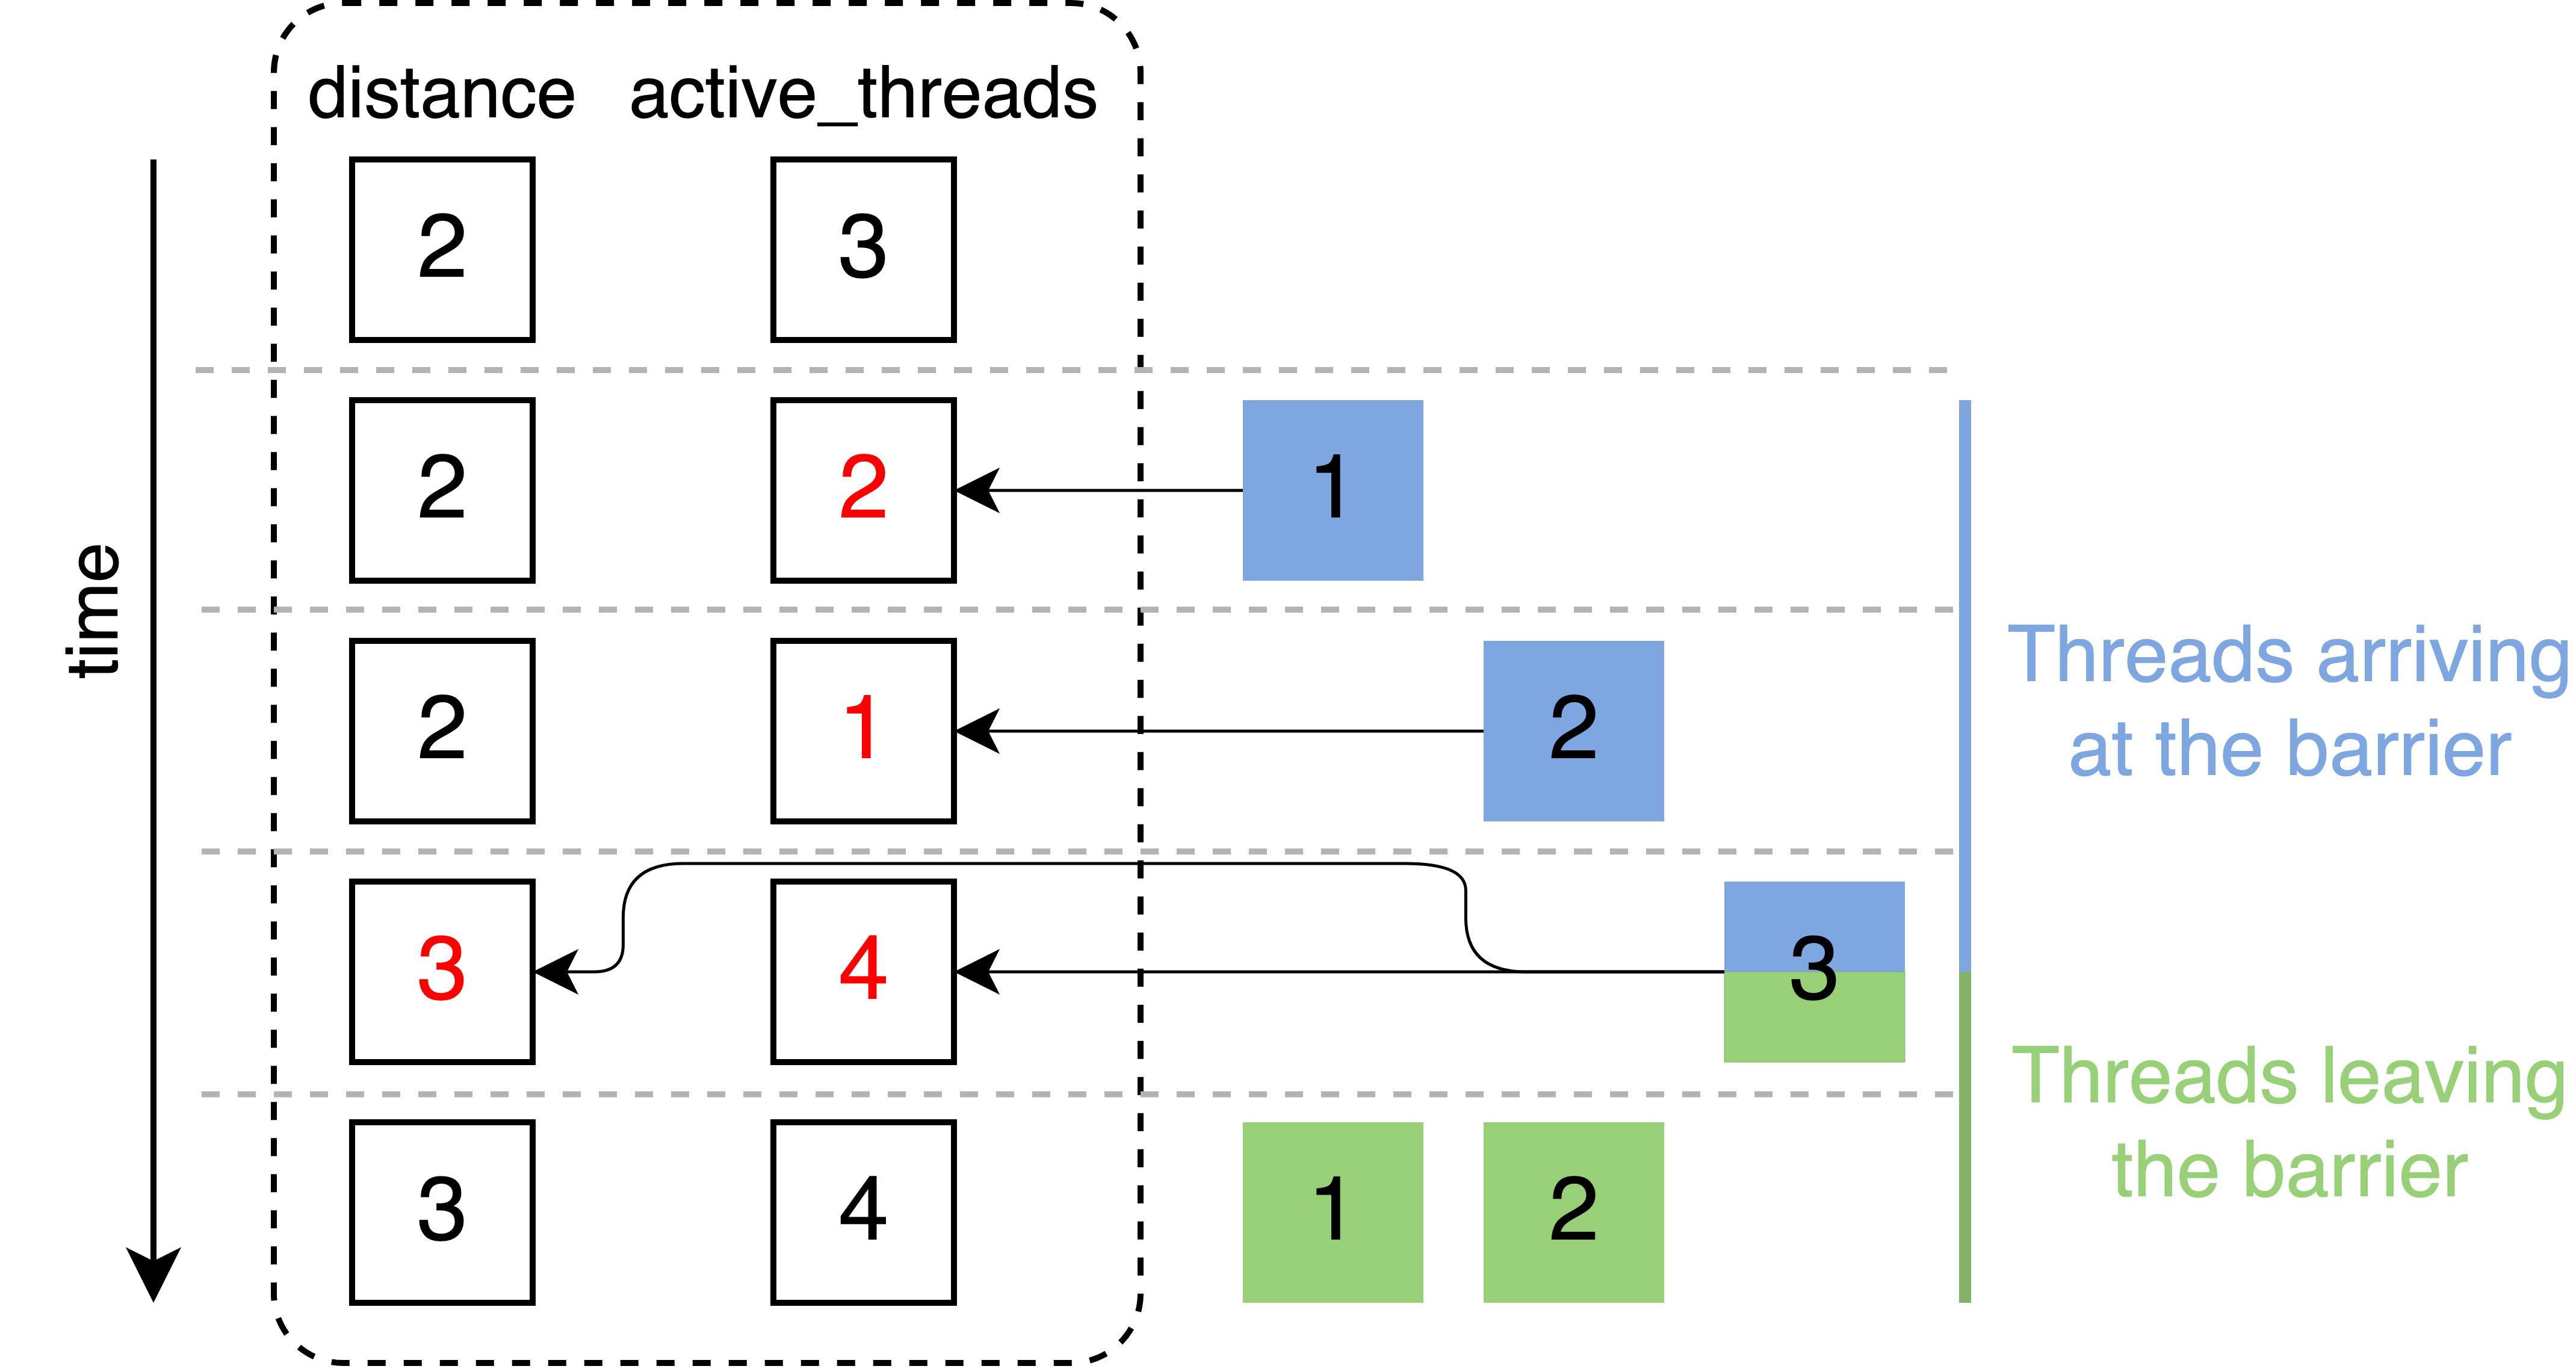
\includegraphics[width=0.6\linewidth]{images/barrier.png}
    \caption{The barrier during a BFS exploration at \texttt{distance = 2} with 3 worker threads. When threads arrive at the barrier (shown in blue), they decrement the \texttt{active\_threads} variable (changes to variables are marked in red) and spin-wait until the \texttt{distance} variable changes. When the last thread arrives at the barrier, it increments the \texttt{distance} and resets \texttt{active\_threads}, thus releasing all the waiting threads (shown in green).}
    \label{fig:barrier}
\end{figure}
\null
\vfill

  \section{Results}
\begin{frame}{Experimental setup}
\begin{itemize}
  \item<1-> Experiments run on 3 platforms:
  \begin{itemize}
    \item AMD EPYC 7543 CPU @ 2.8 GHz (32 cores)
    \item Sophon SG2042 RISC-V CPU @ 2.0 GHz (64 cores)
    \item NVIDIA Grace CPU Superchip @ up to 3.0 GHz (144 cores)
  \end{itemize}
  \item<2-> Datasets: 3 road networks (USA, Europe, Asia), 3 FEM meshes (Earth's crust, steel hook, porous material), 1 random geometric graph (RGG)
  \item<3-> Tools: GCC compiler, Likwid, SBatchMan
  \item<4-> Compared against the GAP benchmark suite
\end{itemize}
\begin{figure}
  \centering
  
\includegraphics[height=1.8cm]{images/tools.png}
\end{figure}
\end{frame}

\begin{frame}{Chunk size impact on performance}
\begin{itemize}
  \item Chunk size determines the number of vertices in a chunk
  \item Chunk sizes of 32 and 64 are optimal for most datasets in multithreaded environments
\end{itemize}
\begin{figure}
  \centering
  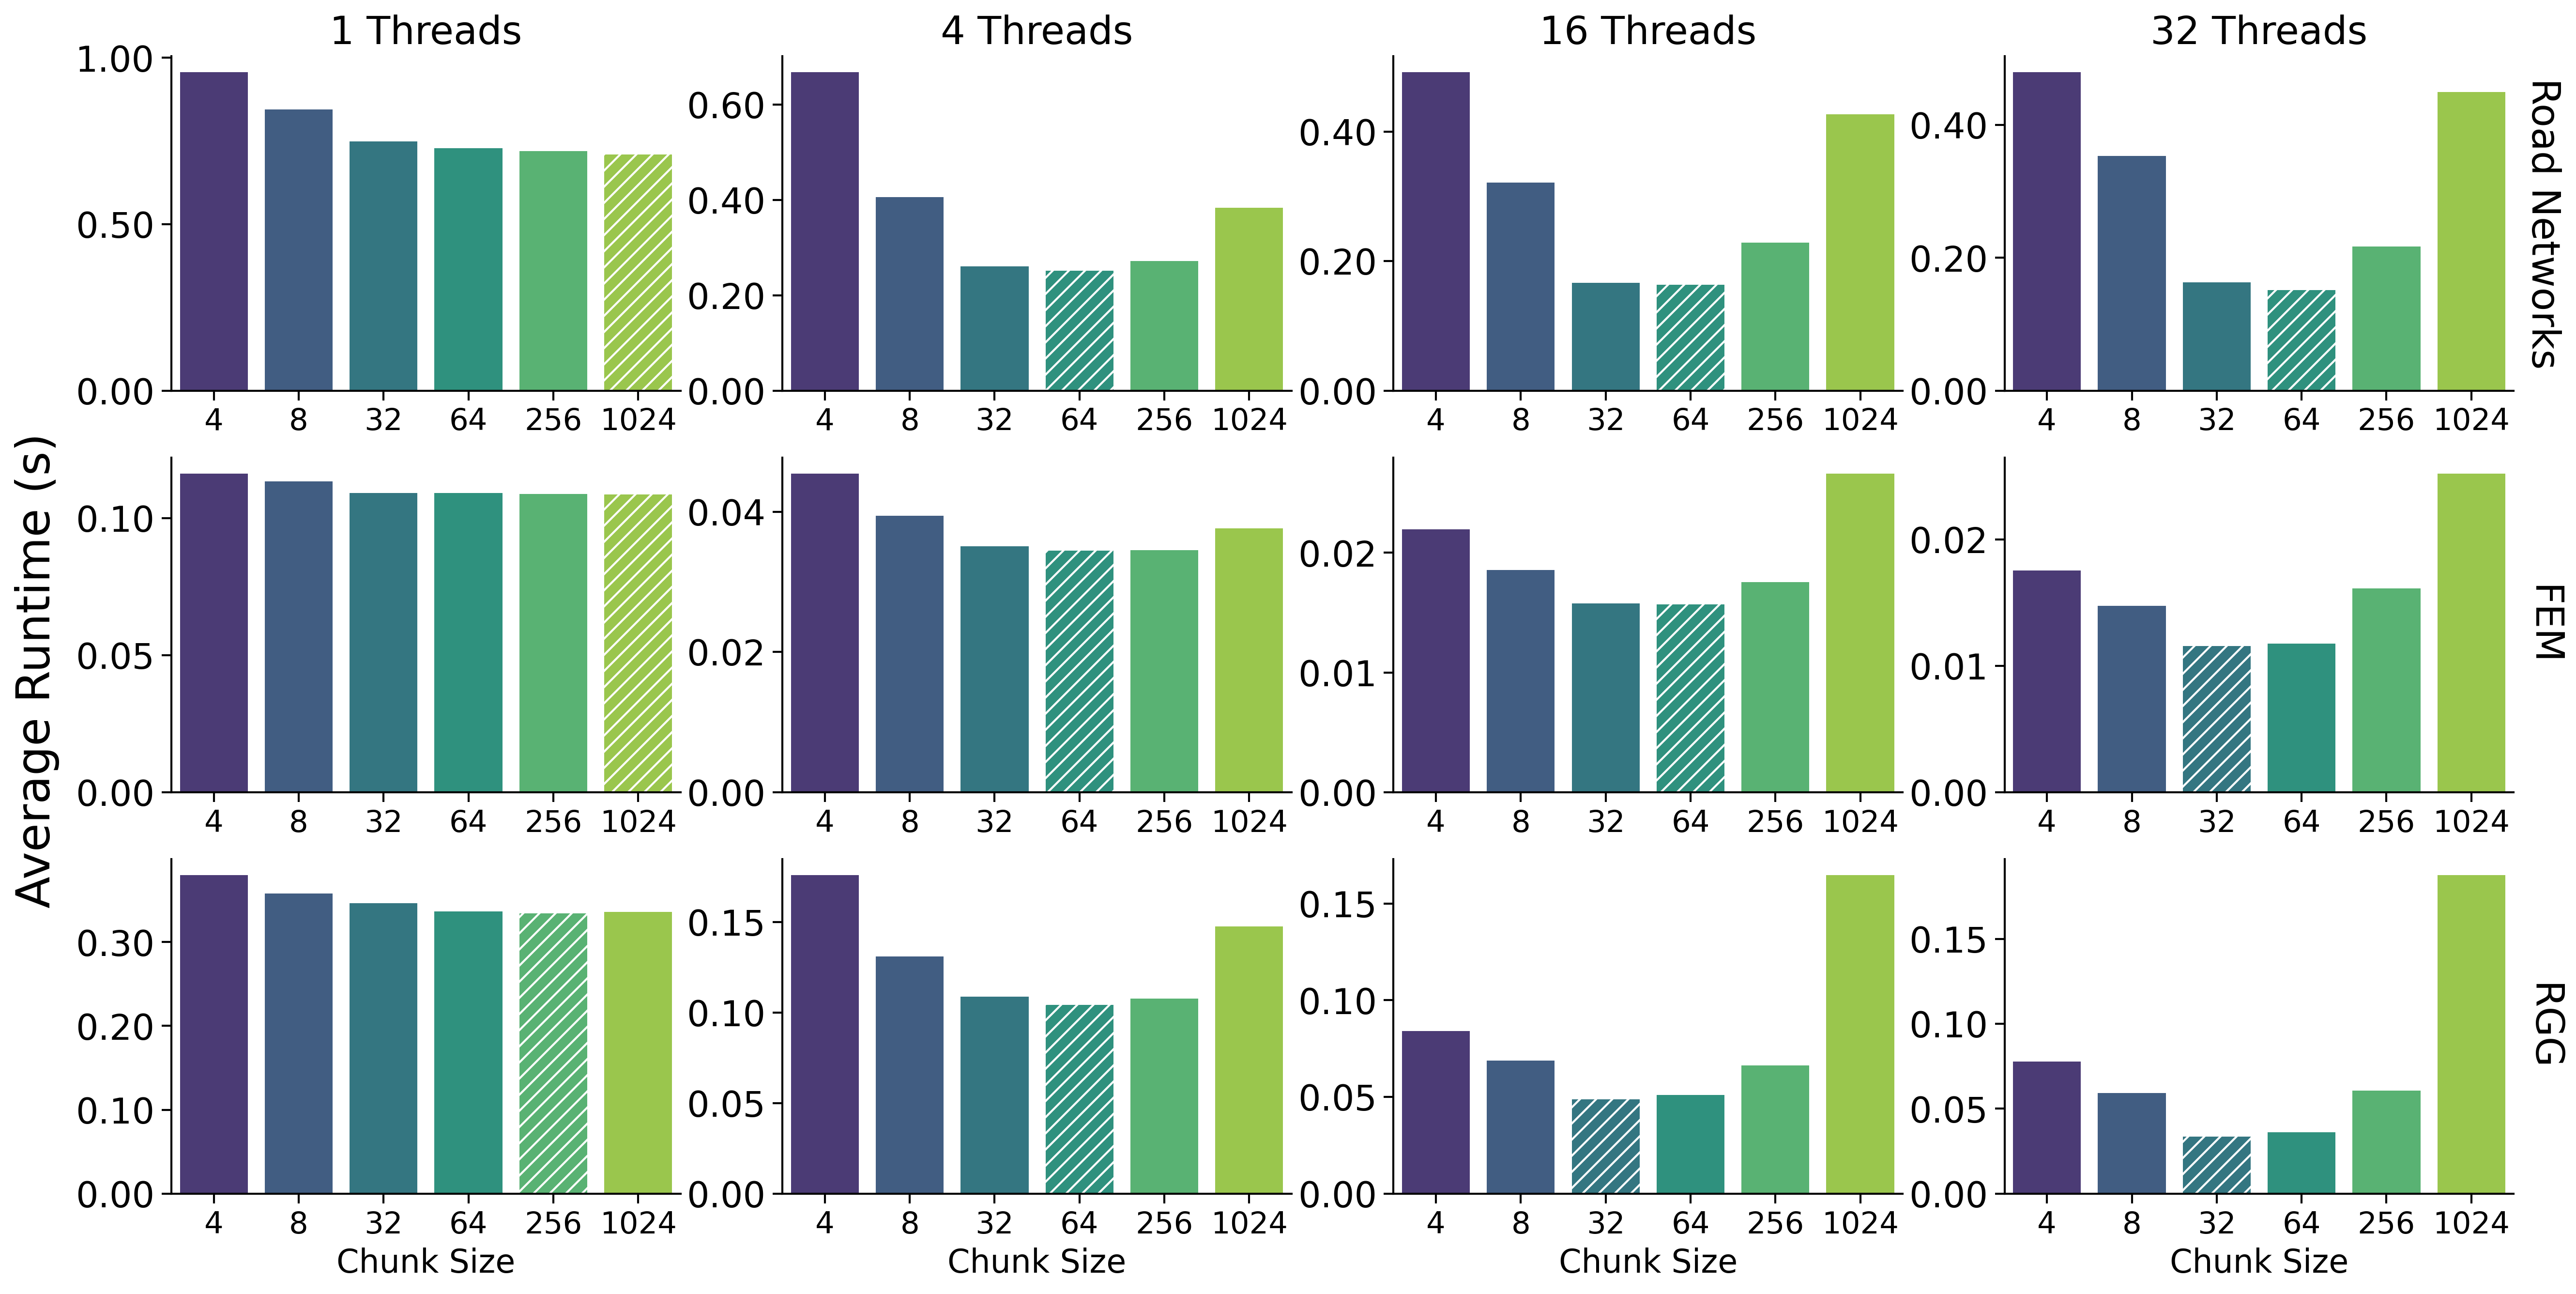
\includegraphics[width=0.8\linewidth]{images/pthreads_chunksize.png}
\end{figure}
\end{frame}

\begin{frame}{Scalability}
\begin{figure}
  \centering
  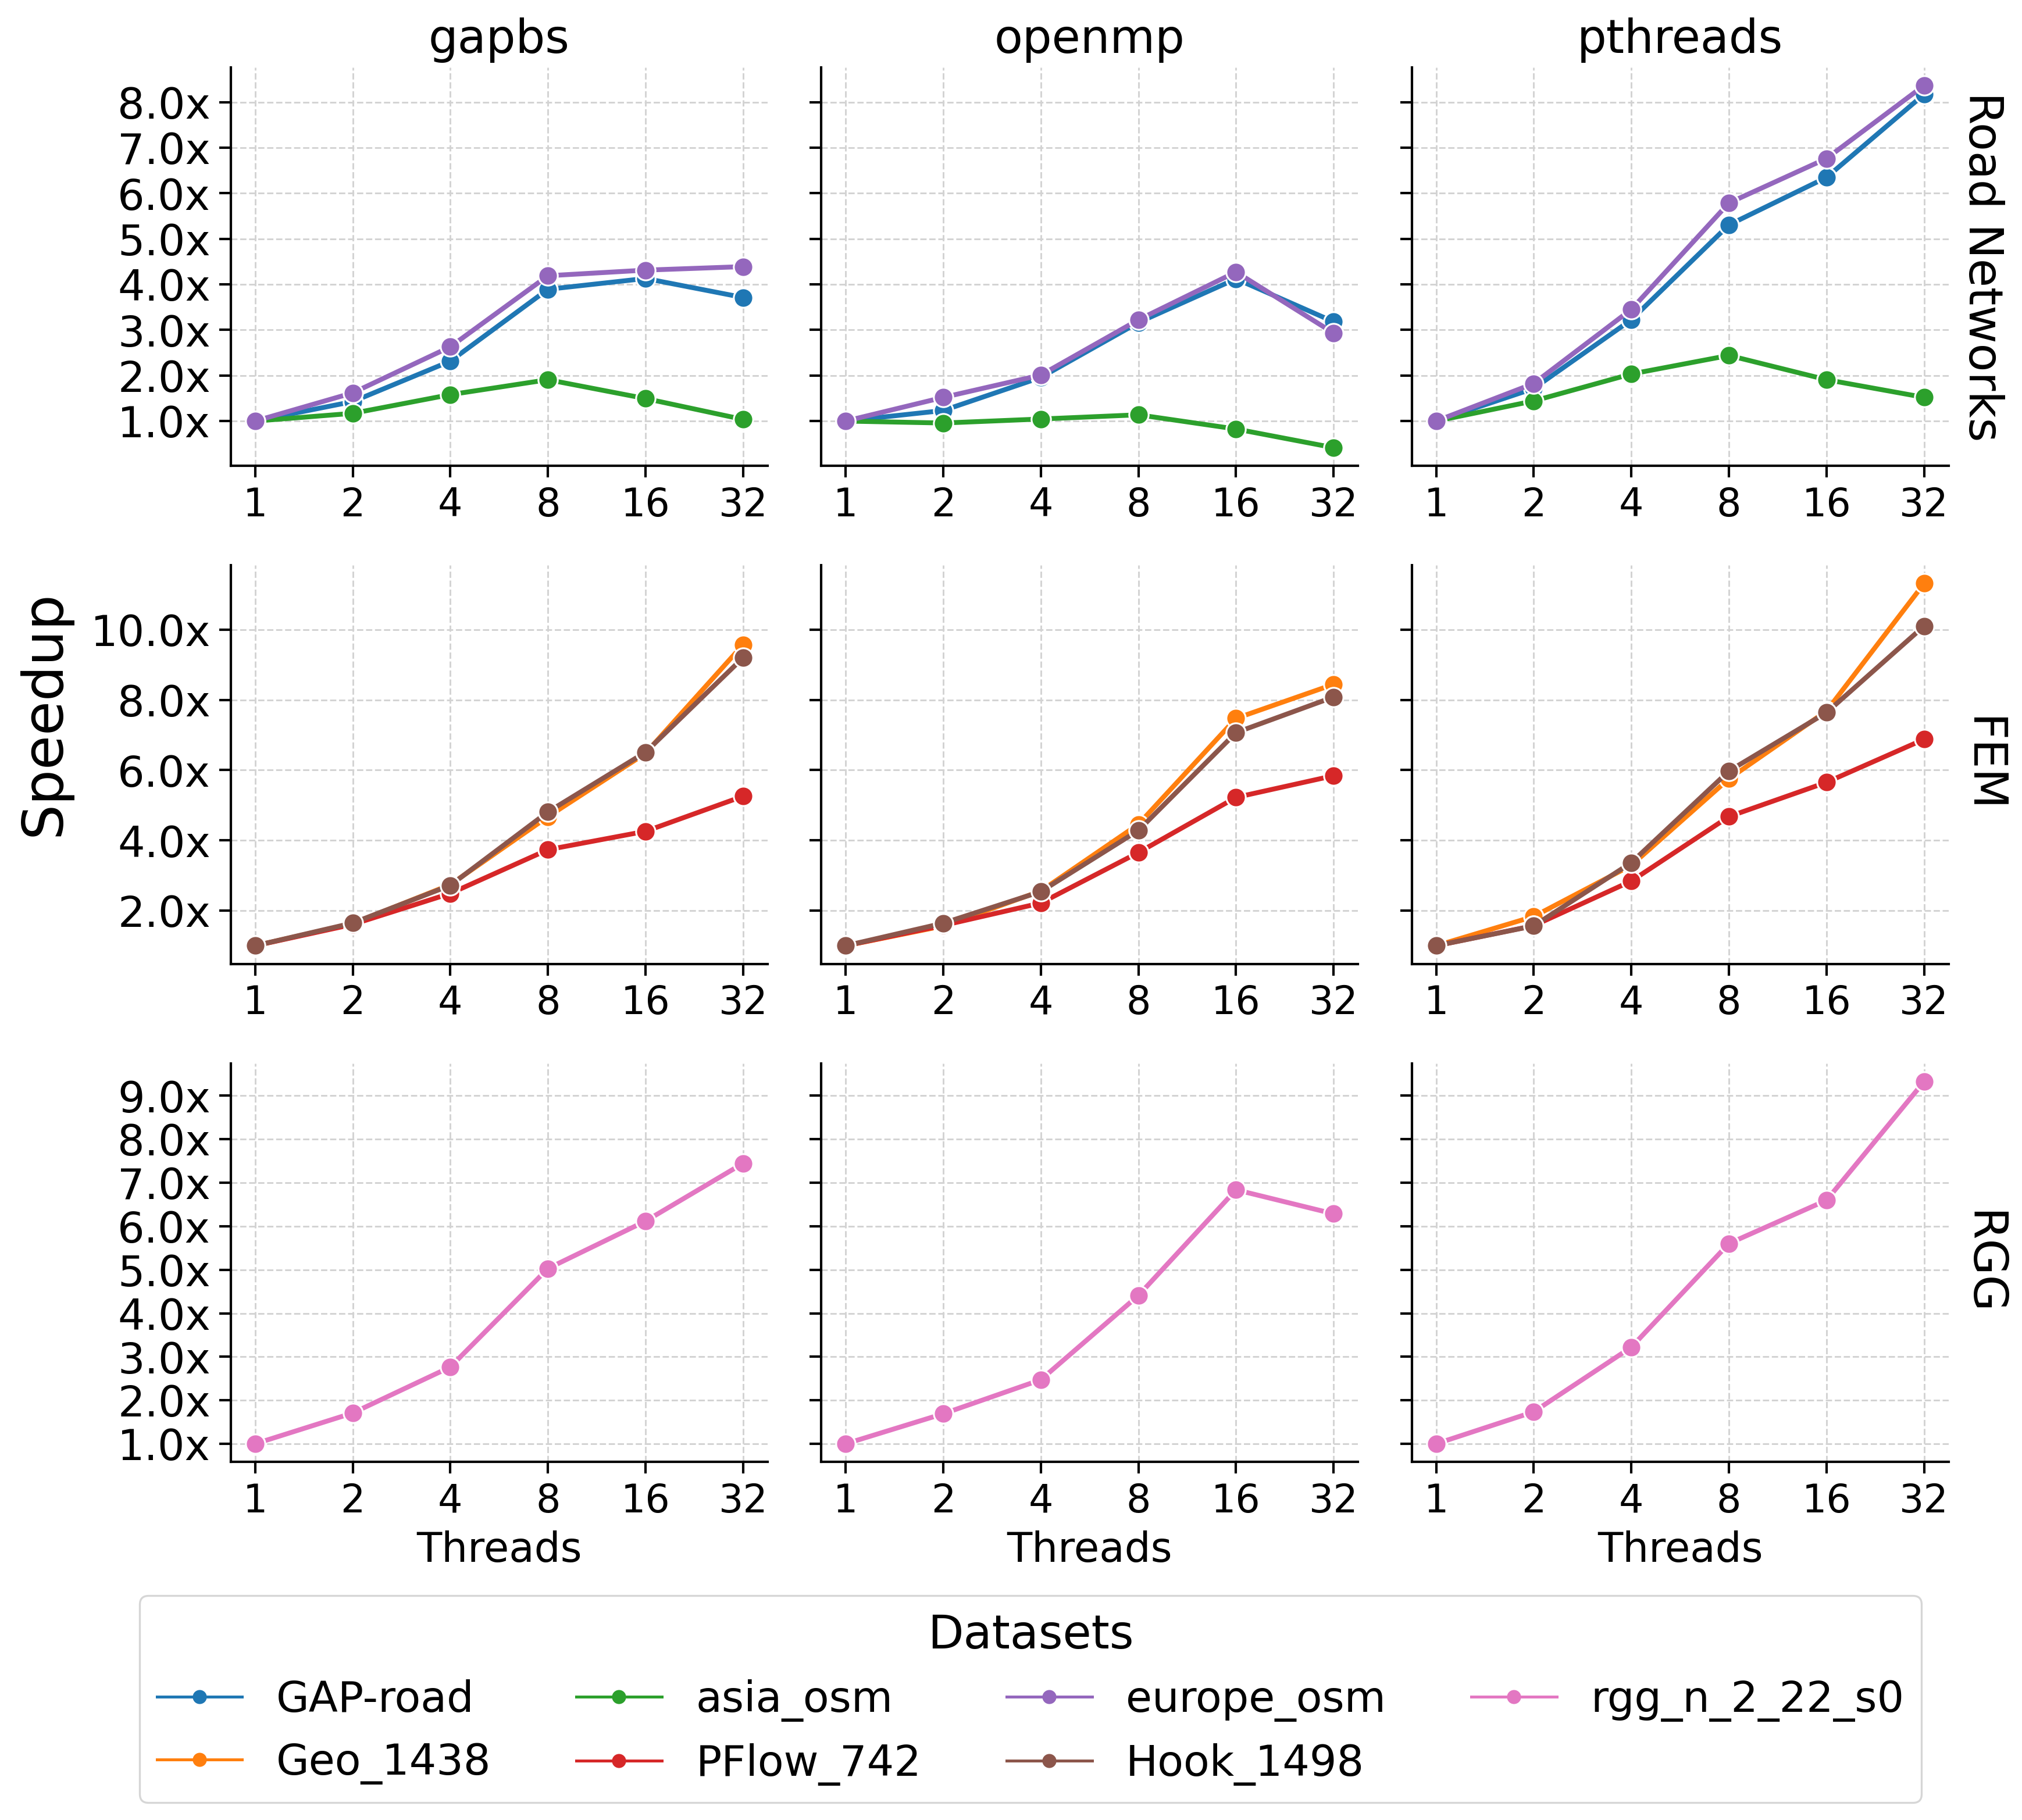
\includegraphics[width=0.6\linewidth]{images/scalability.png}
\end{figure}
\end{frame}

\begin{frame}{Speedup - OpenMP}
\begin{figure}
  \centering
  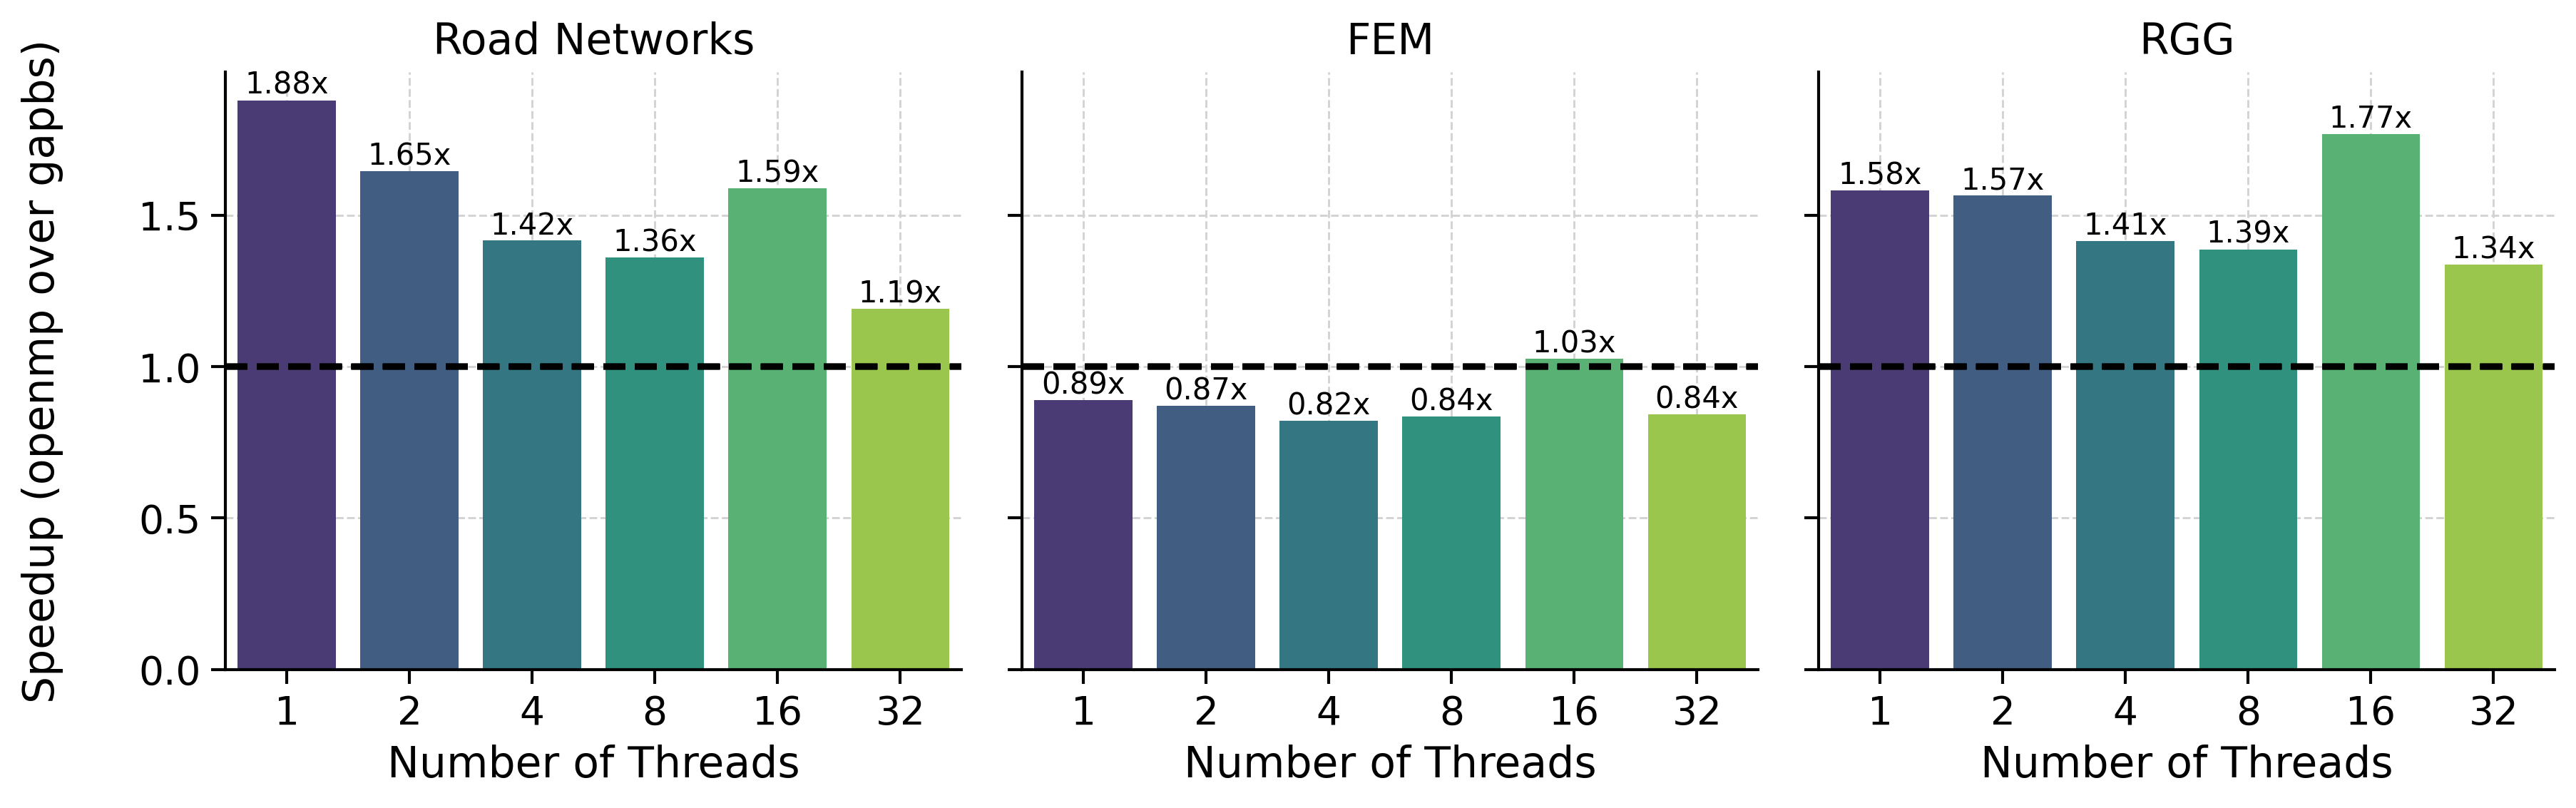
\includegraphics[width=0.8\linewidth]{images/speedup_openmp.png}
  \caption{Speedup of the OpenMP implementation compared to the GAPBS implementation}
\end{figure}
\end{frame}

\begin{frame}{Speedup - Pthreads}
\begin{figure}
  \centering
  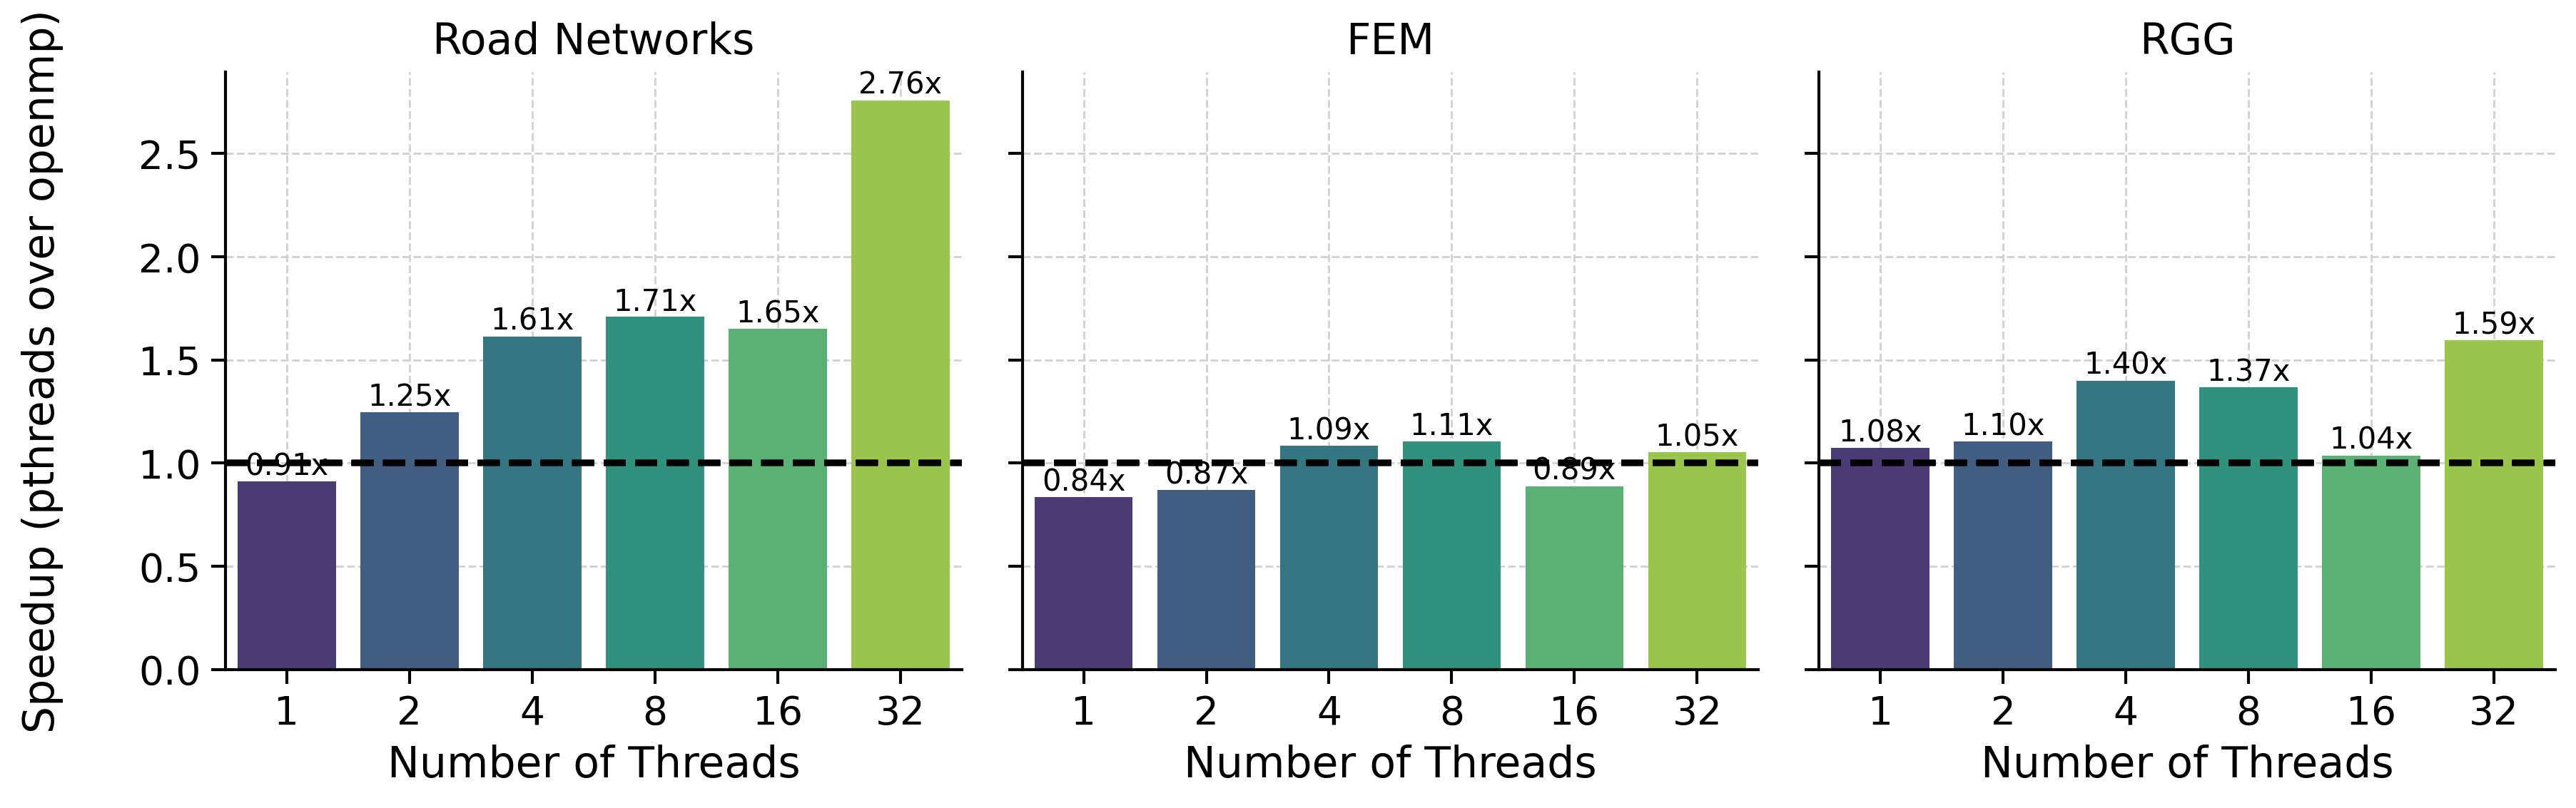
\includegraphics[width=0.8\linewidth]{images/speedup_pthreads.png}
  \caption{Speedup of the pthreads implementation compared to the OpenMP implementation}
\end{figure}
\end{frame}

\begin{frame}{Comparison on different architectures}
\centering
\begin{minipage}{0.8\linewidth}
\begin{figure}
  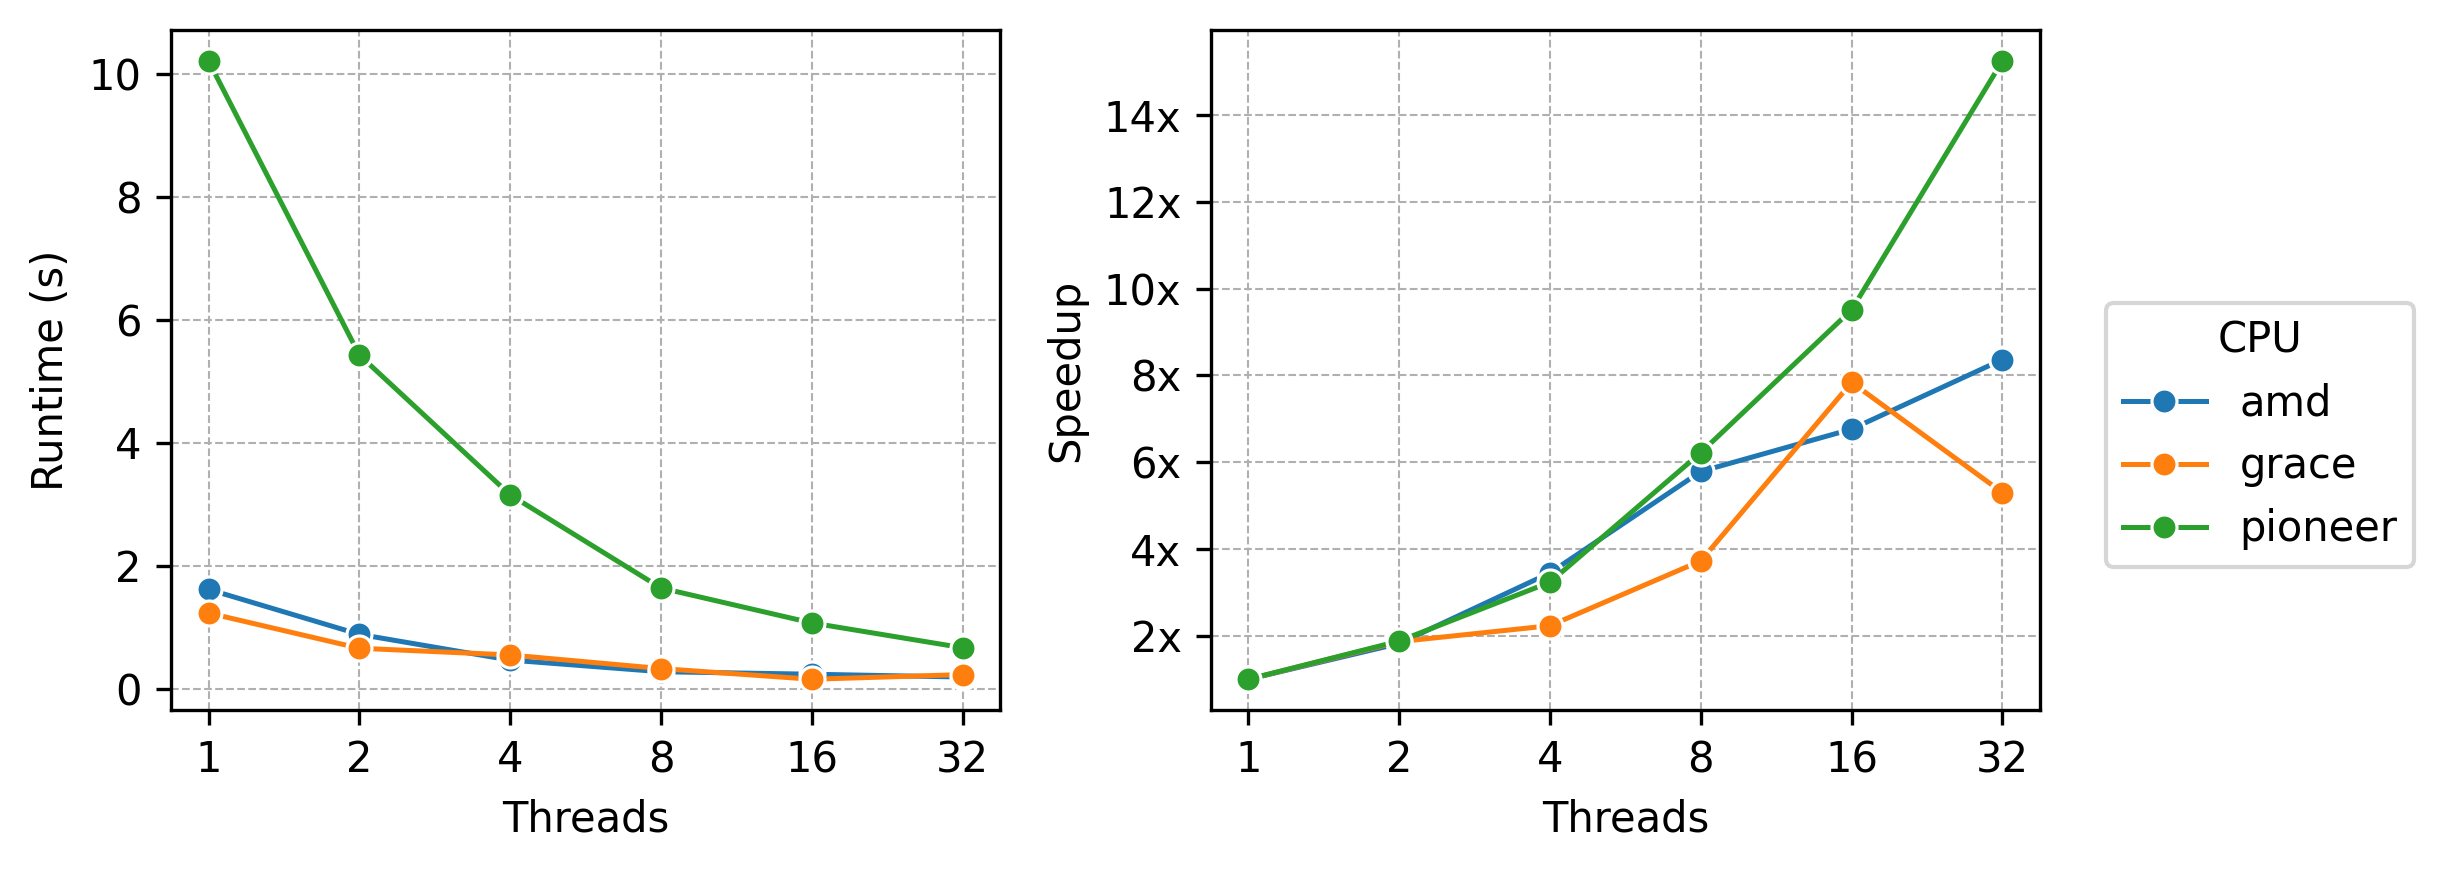
\includegraphics[width=\textwidth]{images/other_platforms.png}
  \caption{\centering Execution time and speedup on different architectures for the Europe road network dataset}
\end{figure}
\end{minipage}
\end{frame}

  % Conclusions
  \chapter{Conclusions}
\label{cha:conclusions}
The efficient execution of Breadth-First Search, a foundational algorithm in graph analytics, is a significant challenge on modern multicore architectures. The primary performance bottleneck is not computational complexity but rather the irregular memory access patterns inherent in traversing large-scale graphs, which leads to poor cache utilization. This thesis addressed this challenge by investigating, implementing, and evaluating two distinct parallel optimization strategies specifically tailored for large-diameter graphs, where the Top-Down traversal approach is most effective. The central hypothesis was that a holistic optimization approach, which considers both the data structure's memory layout and the parallel execution model, is necessary to achieve high performance and scalability.

This work presented two primary contributions. The first was a cache-optimized BFS implementation in C++ using OpenMP, built upon a novel MergedCSR data structure. This format improves spatial locality by co-locating a vertex's metadata directly with its adjacency list. The second contribution was a case study in explicit parallelization, an implementation written in C using the pthreads library. This version provided fine-grained control over the parallel execution model, featuring a persistent thread pool, a dynamic work-stealing mechanism, and a lightweight, custom sense-reversal barrier.

The performance evaluation, conducted across a diverse range of hardware platforms and real-world datasets, yielded several key findings. Firstly, the MergedCSR data structure proved highly effective for purely Top-Down workloads. The OpenMP implementation using this structure achieved a geometric mean speedup of up to 1.5x over the GAP Benchmark Suite baseline on road networks and random geometric graphs, validating the hypothesis that aligning the data structure with the memory hierarchy is critical in performance optimization.

Secondly, the comparative analysis of parallelization strategies revealed the limitations of high-level frameworks for this specific problem domain. While the OpenMP implementation was effective at low core counts, it exhibited negative scaling at higher thread counts due to the overhead of its general-purpose synchronization primitives. In contrast, the explicit pthreads implementation demonstrated superior scalability, achieving a geometric mean speedup of up to 1.55x over the OpenMP version. This finding underscores the importance of a custom parallel execution model for algorithms with fine-grained synchronization. The study also highlighted the limitations of a specialized, Top-Down-only approach, as both implementations were outperformed by the direction-optimizing gapbs on datasets with small-diameter characteristics.

Finally, the evaluation on diverse hardware platforms highlighted the importance of architectural awareness. While the pthreads implementation scaled robustly on the x86-based AMD platform and showed excellent scaling on the RISC-V-based Pioneer board, it suffered from a sharp performance degradation at high core counts on the ARM-based NVIDIA Grace CPU.

Several directions for future research emerge from this work. The most immediate is the extension of these implementations to support a hybrid, direction-optimizing strategy. This would involve adapting the MergedCSR format to support the Bottom-Up traversal's bitmap-based lookups. Another promising direction is the application of these principles, namely, cache-aware data layouts and scalable custom synchronization, to other memory-bound graph algorithms, such as Single-Source Shortest Path or PageRank.

Beyond algorithmic extensions, the OpenMP implementation and the pthreads implementation could serve as a benchmark for evaluating the overhead and scalability of the two parallelization models. Furthermore, for the pthreads implementation, the synchronization mechanisms themselves can be implemented with different primitives, such as atomics or NUMA-aware locks. This modularity allows the implementation to serve as a benchmark for evaluating the performance of these synchronization constructs on different architectures. Also, the existing sense-reversal barrier could be replaced with other mechanisms, such as tree-based or tournament barriers, to analyze how different synchronization strategies interact with a given platform's cache coherence protocol. As demonstrated by the performance difference on the NVIDIA Grace CPU, this approach can reveal performance bottlenecks in both hardware architectures and compiler implementations.

Finally, a more in-depth investigation into the cache behavior using low-level performance counters could further determine the reasons for the observed performance differences. Such an analysis, combined with a direct evaluation of the energy consumption of these implementations, would provide valuable insights, explicitly linking reduced runtimes and fewer memory stalls to improvements in energy efficiency on modern processors.

  \endgroup

  % Bibliography
  \addcontentsline{toc}{chapter}{Bibliography}
  % Alphabetical order of authors
  \bibliographystyle{plain}
  \bibliography{bibliography.bib}

  % Attachments
  %\titleformat{\chapter} {\normalfont\Huge\bfseries}{Appendix \thechapter}{1em}{}
  %\appendix
  %\chapter{Attachment}
\label{cha:attachment}

\end{document}